\documentclass[12pt,a4]{report}
%\documentclass{amsart}
\usepackage{amsmath, amsthm}
\usepackage{amssymb}
\usepackage{amsfonts}
\usepackage{array}
\usepackage{graphicx}% use this package if an eps figure is included.
\usepackage{mathrsfs}
\usepackage{multirow}
\usepackage{siunitx}
\usepackage{accents}
\usepackage{enumerate}
\usepackage{accents,color}
\usepackage{cite}

\setlength\topmargin{-1.1in} \addtolength\textheight{2.1in}
\addtolength{\oddsidemargin}{-0.2in}
\addtolength{\evensidemargin}{-0.1in} \textwidth 5.8in
\newcounter{questioncounter}
\newcounter{equestioncounter}
\setlength\parskip{10pt} \setlength\parindent{0in}
\newcommand{\bea}{\begin{eqnarray*}}
\newcommand{\eea}{\end{eqnarray*}}
\newcommand{\beao}{\begin{eqnarray}}
\newcommand{\eeao}{\end{eqnarray}}
\newcommand{\no}{\noindent}

\theoremstyle{plain}
\newtheorem{theorem}{Theorem}[section]
\newtheorem{example}{Example}[section]
\newtheorem{lemma}[theorem]{Lemma}
\newtheorem{proposition}[theorem]{Proposition}
\newtheorem{corollary}[theorem]{Corollary}
\newtheorem{definition}[theorem]{Definition}
\newtheorem{remark}[theorem]{Remark}


\newcommand{\diam}[0]{\mathrm{diam}}
\newcommand{\rad}[0]{\mathrm{rad}}
\newcommand{\diminf}[0]{\underline{\dim}_B}
\newcommand{\dimsup}[0]{\overline{\dim}_B}
\renewcommand{\Re}[0]{\mathrm{Re}\ }
\renewcommand{\Im}[0]{\mathrm{Im}\ }
\renewcommand{\H}[0]{\mathbb{H}}

%MORE PACKAGES HERE
\newcommand{\R}[0]{\mathbb{R}}
\newcommand{\C}[0]{\mathbb{C}}
\newcommand{\N}[0]{\mathbb{N}}
\newcommand{\Z}[0]{\mathbb{Z}}
\newcommand{\Q}[0]{\mathbb{Q}}
\newcommand{\K}[0]{\mathbb{K}}
\newcommand{\sgn}[0]{\mathrm{sgn}}
\newcommand{\supp}[0]{\mathrm{supp}}

\newcommand{\cred}[1]{{\color{red} #1}}
\newcommand{\cb}[1]{{\color{blue}#1}}

\newcommand{\prodesc}[2]{\left\langle #1 , #2 \right\rangle}





\begin{document}
\title{Multiple Orthogonal Polynomials in several variables}


\author{Fernández, Lidia and Villegas, Juan Antonio\\
\small University of Granada}
\maketitle

\begin{abstract}
\cred{TODO Write the abstract}
\end{abstract}

\section*{Introduction}

Multiple Orthogonality is a theory that extends standard orthogonality. In it, polynomials (defined on the real line in this introduction) satisfy orthogonality relations with respect to more than one measure. There are also two different types of multiple orthogonality, which will be explained shortly.

First, let's consider $r$ different real measures $\mu_1,\dots,\mu_r$ such that $\Omega_j=\supp(\mu_j)\subseteq\R$ ($j=1,\dots,r$). We will use multi-indices $\vec n = (n_1, \dots,n_r)\in \N^r$, and denote $|\vec n| := n_1 + \dots + n_r$. These multi-indices determine the orthogonality relations with each measure. With these preliminaries we will present the first definition.

\begin{definition}[Type II Multiple Orthogonal Polynomials]
    Let $\vec n = (n_1,\dots,n_r)$. A monic polynomial $P_{\vec n}(x)$ is a \textbf{type II multiple orthogonal polynomial} if $\deg(P_{\vec n})= |\vec n|$ and 
    \begin{equation}
        \label{eq:typeII-MOP}
        \int_{\Omega_j} P_{\vec n}(x) x^k d\mu_j(x) = 0, \ \ \ k=0,\dots,n_{j}-1, \ \ j = 1,\dots,r
    \end{equation}
\end{definition}

This means $P_{\vec n}$ is orthogonal to $1,x,x^2,\dots,x^{n_j-1}$ with respect to each measure $\mu_j$, ($j=1,\dots,r$). If we define the inner product 
\begin{equation}
    \label{eq:inner-product}
    \prodesc{f}{g}_j=\int_{\Omega_j}f(x)g(x)d\mu_j(x)
\end{equation}
conditions \eqref{eq:typeII-MOP} can also be written as
\begin{equation}
    \label{eq:typeII-MOP-dot}
    \prodesc{P_{\vec n}}{x^k}_j = 0, \ \ \ k=0,\dots,n_{j}-1, \ \ j = 1,\dots,r
\end{equation}

In addition to type II there exists another type of multiple orthogonality: type I multiple orthogonality.

\begin{definition}[Type I Multiple Orthogonal Polynomials]
    \label{def:typeI-univar}
    Let $\vec n = (n_1,\dots,n_r)$. Type I Multiple Orthogonal Polynomials are presented in a vector $(A_{\vec n, 1}(x), \dots, A_{\vec n, r}(x))$, where $\deg(A_{\vec n, j})\leq n_j-1$, ($j=1,\dots,r$) and these polynomials satisfy
    \begin{equation}
        \label{eq:typeI-MOP}
        \sum_{j=1}^r \int_{\Omega_j}A_{\vec n, j}(x) x^k d\mu_j(x) = 0,  \ \ \ k=0,\dots,|\vec n|-2
    \end{equation}
    and the normalization condition
    \begin{equation}
        \label{eq:typeI-MOP-normalization}
        \sum_{j=1}^r \int_{\Omega_j}A_{\vec n, j}(x) x^{|\vec n|-1} d\mu_j(x) = 1.
    \end{equation}
    
\end{definition}

As we did previously with the type II MOP, the relations \eqref{eq:typeI-MOP} and \eqref{eq:typeI-MOP-normalization} can be written, using the inner products \eqref{eq:inner-product}, as
\begin{equation}
    \label{eq:typeI-MOP-dot}
    \sum_{j=1}^r \prodesc{A_{\vec n,j}}{x^k}_j = \left\{\begin{array}{ccl}
        0 &   \text{ if } & k=0,\dots,|\vec n|-2 \\
        1 & \text{ if } & k=|\vec n|-1      
    \end{array}\right.
\end{equation}

Whenever the measures are all absolutely continuous with respect to a common positive measure $\mu$ defined in $\Omega = \displaystyle\bigcup_{i=1}^r \Omega_i$, \textit{i.e.}, $d\mu_j = w_j(x) d\mu(x)$, ($j=1,\dots,r$), it is possible to define the \textit{Type I function} as
\begin{equation}
    \label{eq:typeI-function}
    Q_{\vec n}(x)=\sum_{j=1}^r A_{\vec n,j}(x)w_j(x).
\end{equation}
Using the type I function, we can rewrite the orthogonality relations
\begin{equation}
    \label{eq:typeI-MOP-function}
    \int_\Omega Q_{\vec n}(x) x^k d\mu(x) = \left\{\begin{array}{ccl}
        0 &   \text{ if } & k=0,\dots,|\vec n|-2 \\
        1 & \text{ if } & k=|\vec n|-1      
    \end{array}\right.
\end{equation}

Nevertheless, not every multi-index $\vec n\in\N^r$ provides a type I vector of polynomials or a type II polynomial. Let $\vec n = (n_1,\dots,n_r)$ be a multi-index and let $\mu_1,\dots,\mu_r$ be $r$ positive measures. If $(A_{\vec n, 1}(x), \dots, A_{\vec n, r}(x))$ is a vector of type I MOP, then, if we denote
\begin{equation}
    \begin{split}
        A_{\vec n,1}(x) &= a_{n_1-1,1}x^{n_1-1} + a_{n_1-2,1}x^{n_1-2} + \cdots + a_{1,1}x + a_{0,1} \\
        \vdots & \\
        A_{\vec n,r}(x) &= a_{n_r-1,r}x^{n_r-1} + a_{n_r-2,r}x^{n_r-2} + \cdots + a_{1,r}x + a_{0,r}
    \end{split}
\end{equation}
and apply the orthogonality conditions \eqref{eq:typeI-MOP} and \eqref{eq:typeI-MOP-normalization}, then we get a linear system of $|\vec n|$ equations and $|\vec n|$ unknown coefficients. Thus, the type I MOP will exist and it will be unique if and only if the following matrix is regular:

\begin{equation}
    \label{eq:MOP-matrix}
    A=\left(\begin{array}{c}
    M_{n_1}^{(1)} \\ \hline
    M_{n_2}^{(2)} \\ \hline
    \vdots \\ \hline
    M_{n_r}^{(r)} \\ 
\end{array}\right), \text{ \ \  where \ \ } M_{n_j}^{(j)} = \begin{pmatrix}
    m_0^{(j)} & m_1^{(j)} & \cdots & m_{n-1}^{(j)} \\
    m_1^{(j)} & m_2^{(j)} & \cdots & m_{n}^{(j)} \\
    \vdots & \vdots & \ddots & \vdots \\
    m_{n_j-1}^{(j)} & m_{n_j}^{(j)} & \cdots & m_{n+n_j-2}^{(j)} \\
\end{pmatrix},
\end{equation}
$j=1,\dots,r$ and $m_k^{(j)}=\displaystyle\int_{\Omega_j} x^k d\mu_j(x)$ are the moments of the measures $(k\geq 0)$.

On the other hand, if we consider the type II polynomial as:
$$
P_{\vec n} = x^{|\vec n|} + a_{|\vec n|-1} x^{|\vec n|-1} + \cdots + a_1 x + a_0
$$
and apply the conditions \eqref{eq:typeII-MOP}, we get another linear system with $|\vec n|$ equations and $|\vec n|$ unknown coefficients. In fact, the coefficient matrix of this linear system is $A^t$, the transpose matrix of the type I MOP. Thus, we have the following result.

\begin{proposition}
    \label{prop:existence-of-MOP}
    Given a multi-index $\vec n\in\N^r$ and $r$ positive measures, $\mu_1,\dots,\mu_r$, the following statements are equivalent:
    \begin{enumerate}
        \item There exist a unique vector $(A_{\vec n,1}, \dots, A_{\vec n,r})$ of type I MOP.
        \item There exist a unique type II multiple orthogonal polynomial $P_{\vec n}$.
        \item The matrix $A$ defined in \eqref{eq:MOP-matrix} is regular.
    \end{enumerate}
\end{proposition}

Following this proposition, we provide a new definition.

\begin{definition}
    A multi-index $\vec n = (n_1,\dots,n_r)\in\N^r$ is \textbf{normal} if it satisfies the conditions of Proposition \ref{prop:existence-of-MOP}.
    A system of $r$ measures $\mu_1,\dots,\mu_r$ is \textbf{perfect} if every $\vec n\in\N^r$ is normal.
\end{definition}

There are some perfect systems, standing out the Angelesco systems and the AT-systems, see \cite[Sections 23.1.1 and 23.1.2]{Ismail}

We will be mainly focused on type II multiple orthogonal polynomials. In next sections, a definition of type II multiple orthogonal polynomials on several variables will be provided, along with a few simple examples and a generalized version of the Jacobi-Piñeiro polynomials. 
\cred{REVIEW No poner esto en el poster que los piñeiro no ha dado la vida}

\section*{Orthogonal Polynomials Systems in several variables}

First of all, we introduce the notation that will be used. Let $\Pi^d=\R[x_1,\dots,x_d]$ be the space of polynomials in $d$ variables. If $d=2$, we use the variables $x,y$. For $n\in\N_0$, the space generated by all the degree $n$ monomials is denoted by 
$$
\mathcal{P}_n^d = \left\langle x_1^{k_1} x_2^{k_2} \cdots x_d^{k_d}: k_1+k_2+\cdots +k_d = n, k_1,k_2,\dots,k_d\in\N_0\right\rangle
$$
It is possible to check by induction that the number of different monomials of degree $n$ with $d$ variables is $\displaystyle\binom{n+d-1}{n}$. So, this means
$$
\dim \mathcal{P}_n^d = \binom{n+d-1}{n}.
$$

In order to work with multivariate polynomials, we will use the notation $\mathbb P_n$ as a column polynomial vector. In order to understand this notation, we denote the vector of degree $j$ monomials as
$$
\mathbb{X}_j = \left(x_1^{k_1} x_2^{k_2} \cdots x_d^{k_d}\right)_{k_1+k_2+\cdots +k_d = j}.
$$
For example, if $d=2$ and we use the ``degree reverse lexicographic ordering'' in $\N^2$, then
$$
\mathbb{X}_0=\left(1\right), \mathbb{X}_1=\begin{pmatrix}
    x \\ y
\end{pmatrix}, \mathbb{X}_2=\begin{pmatrix}
    x^2 \\ xy \\ y^2
\end{pmatrix}, \dots, \mathbb{X}_j=\begin{pmatrix}
    x^j \\ x^{j-1}y \\ \vdots \\ y^j
\end{pmatrix}.
$$
Thus, a column polynomial vector of degree $n$ can be represented as
$$
\mathbb{P}_n = G_{n,n}\mathbb{X}_n + G_{n,n-1}\mathbb{X}_{n-1}+\cdots G_{n,1}\mathbb{X}_1 + G_{n,0}\mathbb X_0,
$$
where $G_{n,j}$ are matrices of size $\binom{n+d-1}{n}\times\binom{j+d-1}{j}$ and they are the polynomial's ``coefficients''. Hence, $\mathbb P_n$ is a vector of polynomials of size $\binom{n+d-1}{n}$. We denote 
$$
r_n^d = \dim \mathcal{P}_n^d = \binom{n+d-1}{n}.
$$

Given a multi-dimensional measure $\mu(x_1,\dots,x_d)$, with support $\Omega\subseteq\R^d$, we can extend the definition of a multivariate product $\prodesc{f}{g}_\mu$ and its functional $\mathcal{L}_\mu[f\cdot g]$ to column vectors. If $F=(f_1,f_2,\dots,f_n)^t$ and $G=(g_1,g_2,\dots, g_m)^t$ are column vectors of functions of size $n$ and $m$, respectively, then we define
\begin{equation}
    \label{eq:prodesc-matrix}
    \prodesc{F}{G}:=\mathcal{L}_\mu[F\cdot G^T] = \int_\Omega F\cdot G^T d\mu(x_1,\dots,x_d) = \left(\int_\Omega f_i\cdot g_j d\mu(x_1,\dots,x_d)\right)_{i,j=1}^{n,m}.
\end{equation}

\cred{REVIEW como pongo esto para que salga en forma de matriz :(}

In fact, we are applying the standard product $\prodesc{f_i}{g_j}_\mu$ or the functional $\mathcal L_\mu[f_i\cdot g_j]$ to each pair $i,j$ and placing the results in a matrix.

Let $\{\mathbb{P}_n\}_{n\geq 0}$ be a system of polynomial vectors such that
$$
\prodesc{\mathbb P_n}{\mathbb P_k}_\mu = \mathcal{L}_\mu[\mathbb P_n \mathbb P_k^t]= \left\{\begin{array}{ccl}
    0_{r_n^d\times r_k^d} &   \text{ if } & k=0,\dots,n-1 \\
    S_n & \text{ if } & k=n      
\end{array}\right. 
$$
Where $S_n$ is a regular squared matrix of size $r_n^d\times r_n^d$.
Due to orthogonality, it is possible to give an equivalent condition:
\begin{equation}
    \label{eq:prodesc-matrix-PX}
    \prodesc{\mathbb P_n}{\mathbb X_k}_\mu = \mathcal{L}_\mu[\mathbb P_n \mathbb X_k^t]= \left\{\begin{array}{ccl}
        0_{r_n^d\times r_k^d} &   \text{ if } & k=0,\dots,n-1 \\
        S_n & \text{ if } & k=n      
    \end{array}\right. 
\end{equation}
Then, $\{\mathbb{P}_n\}_{n\geq 0}$ is called a system of orthogonal polynomials with respect to the measure $\mu$ or the functional $\mathcal L_\mu$. Further information about this topic is available in \cite[Ch. III, Section 3.2]{dunkl_xu_2014}.

\chapter{First approach: Bivariate Multiple Orthogonal Polynomial Vectors}

\section{Type II MOP in several variables}

In order to give a definition of type II orthogonality, we will take as a reference the definition of type II orthogonality in the univariate case. given $r\in\N$, $\vec n = (n_1,\dots, n_r)\in\N^r$, $r$ $d$-dimensional measures $\mu_1, \dots, \mu_r$ and their respective matrix inner products defined in \eqref{eq:prodesc-matrix}, we are going to define the type II multiple orthogonal polynomial vector as a monic polynomial vector $\mathbb P_{\vec n} = \mathbb X_n + \displaystyle\sum_{k=0}^{n-1}G_{n,k} \mathbb X_k$ which satisfies
\begin{equation}
    \label{eq:typeII-MOP-d-variables}
    \prodesc{\mathbb P_{\vec n}}{\mathbb X_k}_i = 0, \ \ \ k=0,\dots,n_i-1, \ \ \ i=1,\dots,r
\end{equation}
Note the similarity between conditions \eqref{eq:typeII-MOP-dot} and \eqref{eq:typeII-MOP-d-variables}. However, when we work with one variable, it is known type II polynomial is a monic polynomial whose degree is exactly $|\vec n|$. This is because the number of coefficients of a degree $|\vec n|$ univariate monic polynomial ($|\vec n|$) is equal to both the number of orthogonality conditions and the size of matrices $A$ defined in \eqref{eq:MOP-matrix}. Due to the differences between univariate and multivariate case, the degree $n$ of a polynomial vector $\mathbb P_{\vec n}$ might not be equal to $|\vec n|$. For now, this degree $n$ will be considered as unknown, getting to know it later.

As mencioned above, in the univariate multiple orthogonality, $\deg(P_{\vec n})=|\vec n|$. The main reason why this happens is because the condition $\prodesc{P_{\vec n}}{x^k}=0$ is a linear equation (only one). Hence, we are looking for a polynomial with $|\vec n|$ unknown coefficients and we have $|\vec n|$ linear equations deduced from conditions \eqref{eq:typeII-MOP-dot}. Then, it is possible to build a system of linear equations with coefficient matrix $A^t$ given in \eqref{eq:MOP-matrix}.

If we work with $d$ variables, attending to \eqref{eq:prodesc-matrix-PX}, $\prodesc{\mathbb P_{\vec n}}{\mathbb X_k}$ is a matrix of size $r_n^d\times r_k^d$. Then, equation $\prodesc{\mathbb P_{\vec n}}{\mathbb X_k}_i = 0$ gives us $r_n^d\times r_k^d$ linear equations.

Now, the question is: How many linear equations is it possible to get from a multi-index $\vec n =(n_1, \dots, n_r)$? The answer to this problem is easy since, if we fix $j\in\{1,\dots,r\}$:
\begin{itemize}
    \item $\prodesc{\mathbb P_{\vec n}}{\mathbb X_0}_j = 0_{r^d_n\times r^d_0}$, we get $r^d_n\times r^d_0$ equations.
    \item $\prodesc{\mathbb P_{\vec n}}{\mathbb X_1}_j = 0_{r^d_n\times r^d_1}$, we get $r^d_n\times r^d_1$ equations.
    \item \dots
    \item $\prodesc{\mathbb P_{\vec n}}{\mathbb X_{n_j-1}}_j = 0_{r^d_n\times r^d_{n_i-1}}$, we get $r^d_n\times r^d_{n_j-1}$ equations.
\end{itemize} 
If we collect all the equations, we obtain $r_n^d\cdot\displaystyle\sum_{k=0}^{n_j-1}r^d_k$ linear equations for each $j\in\{1,\dots,r\}$. Collecting the number of equations of each $j$, we finally get that the number of equations is 
\begin{equation}
    \label{eq:number-eqs}
    r_n^d \sum_{j=1}^r \sum_{k=0}^{n_j-1} r_k^d.
\end{equation}

On the other hand, since $\mathbb P_{\vec n} = \mathbb X_n + \displaystyle\sum_{k=0}^{n-1}G_{n,k} \mathbb X_k$, where $G_{n,k}$ are matrices of dimensions $r^d_n\times r^d_k$, if we consider $\mathbb P_{\vec n}$ a vector of degree $n$ monic polynomials, then this matrices give us $\displaystyle\sum_{k=0}^{n-1}r^d_n r^d_k=r^d_n\displaystyle\sum_{k=0}^{n-1} r^d_k$ unknown coefficients.

We want this system to have only one unique solution for a multi-index $\vec n$. Then, we will say $\vec n$ is an $n$-\textbf{admissible} multi-index if there exist a number $n\in\N_0$ such that:
\begin{equation}
    \label{eq:condition-type-ii-general}
    \displaystyle\sum_{k=0}^{n-1} r^d_k = \sum_{i=1}^r \sum_{k=0}^{n_i-1} r_k^d.
\end{equation}
This number $n$ is the degree of type II polynomials. In order to emphasise the degree of the polynomials, in the next sections we denote type II MOP as $\mathbb P_{\vec n}^n$.

\cb{REVIEW No me termina de hacer gracia el concepto de admisible porque al final está relacionado con un número $n$. A la hora de hablar de que un multi-indice es admisible lo suyo es decir después para qué $n$. He pensado que quizá estaría bien decir que es $n$-admisible?}

\section{The bidimensional case}

From now on, we will assume $d=2$ and $x:=x_1, y:=x_2$. Notice that, in the bidimensional case, $r^2_n = \binom{n+1}{n} = n+1$, which makes things much easier: $\mathbb X_j$ is a polynomial vector of size $j+1$, $\mathbb P_n$ is a vector of size $n+1$, and $G_{n,k}$ is a $(n+1)\times(k+1)$ matrix. Also, condition \eqref{eq:condition-type-ii-general} gets simpler because some sums become sums of arithmetic progressions. When $d=2$, a multi-index $\vec n =(n_1,\dots,n_r)$ is $n$-admissible if there exists a number $n\in\N\cup \{0\}$ such that
\begin{equation}
    \label{eq:condition-type-ii}
    n(n+1)=\sum_{j=1}^r n_j (n_j+1).
\end{equation} 

Observe some of the admissible multi-indices and their respective degree $n$ in tables \ref{tab:2measuresindices} and \ref{tab:3measuresindices}, and a visual representation of some of them when $r=2$ and $r=3$ in figure \ref{fig:indices}.

\begin{table}[h]
    \centering
    \begin{tabular}{|c|c|}
    \hline
    $n$ & admissible multi-indices when $r=2$ and $d=2$ \\ \hline
    $0$ & $(0,0)$                                  \\ \hline
    $1$ & $(0,1), (1,0)$                           \\ \hline
    $2$ & $(0, 2), (2, 0)$                         \\ \hline
    $3$ & $(0, 3), (2, 2), (3, 0)$                 \\ \hline
    $4$ & $(0, 4), (4, 0)$                         \\ \hline
    $5$ & $(0, 5), (5, 0)$                         \\ \hline
    $6$ & $(0, 6), (3, 5), (5, 3), (6, 0)$         \\ \hline
    $7$ & $(0, 7), (7, 0)$                         \\ \hline
    $8$ & $(0, 8), (5, 6), (6, 5), (8, 0)$         \\ \hline
    $9$ & $(0, 9), (9, 0)$                         \\ \hline
    \end{tabular}
    \caption{Admissible multi-indices when using $r=2$ measures}
    \label{tab:2measuresindices}
\end{table}

\begin{table}[]
    \centering
    \begin{tabular}{|c|c|}
    \hline
    $n$ & admissible multi-indices when $r=3$ and $d=2$                                                                                                                                                                           \\ \hline
    $0$ & $(0,0,0)$                                                                                                                                                                                                          \\ \hline
    $1$ & $(0, 0, 1), (0, 1, 0), (1, 0, 0)$                                                                                                                                                                                  \\ \hline
    $2$ & $(0, 0, 2), (0, 2, 0), (1, 1, 1), (2, 0, 0)$                                                                                                                                                                       \\ \hline
    $3$ & $(0, 0, 3), (0, 2, 2), (0, 3, 0), (2, 0, 2), (2, 2, 0), (3, 0, 0)$                                                                                                                                                 \\ \hline
    $4$ & $(0, 0, 4), (0, 4, 0), (1, 2, 3), (1, 3, 2), (2, 1, 3), (2, 3, 1), (3, 1, 2), (3, 2, 1), (4, 0, 0)$                                                                                                                \\ \hline
    $5$ & $(0, 0, 5), (0, 5, 0), (2, 3, 3), (3, 2, 3), (3, 3, 2), (5, 0, 0)$                                                                                                                                                 \\ \hline
    $6$ & \begin{tabular}[c]{@{}c@{}}$(0, 0, 6), (0, 3, 5), (0, 5, 3), (0, 6, 0), (1, 4, 4), (2, 2, 5), (2, 5, 2), (3, 0, 5),$ \\ $(3, 5, 0), (4, 1, 4), (4, 4, 1), (5, 0, 3), (5, 2, 2), (5, 3, 0), (6, 0, 0)$\end{tabular} \\ \hline
    $7$ & \begin{tabular}[c]{@{}c@{}}$(0, 0, 7), (0, 7, 0), (1, 3, 6), (1, 6, 3), (2, 4, 5), (2, 5, 4), (3, 1, 6), (3, 6, 1),$ \\ $(4, 2, 5), (4, 5, 2), (5, 2, 4), (5, 4, 2), (6, 1, 3), (6, 3, 1), (7, 0, 0)$\end{tabular} \\ \hline
    $8$ & \begin{tabular}[c]{@{}c@{}}$(0, 0, 8), (0, 5, 6), (0, 6, 5), (0, 8, 0), (3, 5, 5), (5, 0, 6), (5, 3, 5), (5, 5, 3),$ \\ $(5, 6, 0), (6, 0, 5), (6, 5, 0), (8, 0, 0)$\end{tabular}                                  \\ \hline
    $9$ & \begin{tabular}[c]{@{}c@{}}$(0, 0, 9), (0, 9, 0), (2, 3, 8), (2, 6, 6), (2, 8, 3), (3, 2, 8), (3, 8, 2), (5, 5, 5), (6, 2, 6),$ \\ $(6, 6, 2), (8, 2, 3), (8, 3, 2), (9, 0, 0)$\end{tabular}                       \\ \hline
    \end{tabular}
    \caption{Admissible multi-indices when using $r=3$ measures}
    \label{tab:3measuresindices}
    \end{table}
    
    \begin{figure}[h]
        \centering\begin{tabular}{cc}
          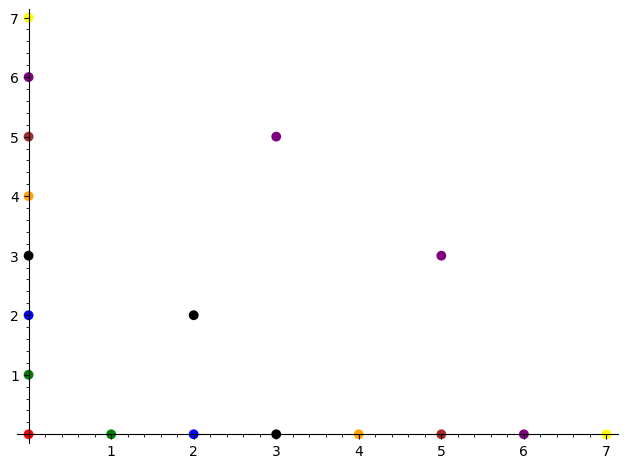
\includegraphics[height=5cm]{./img/puntos2D.png} & 
          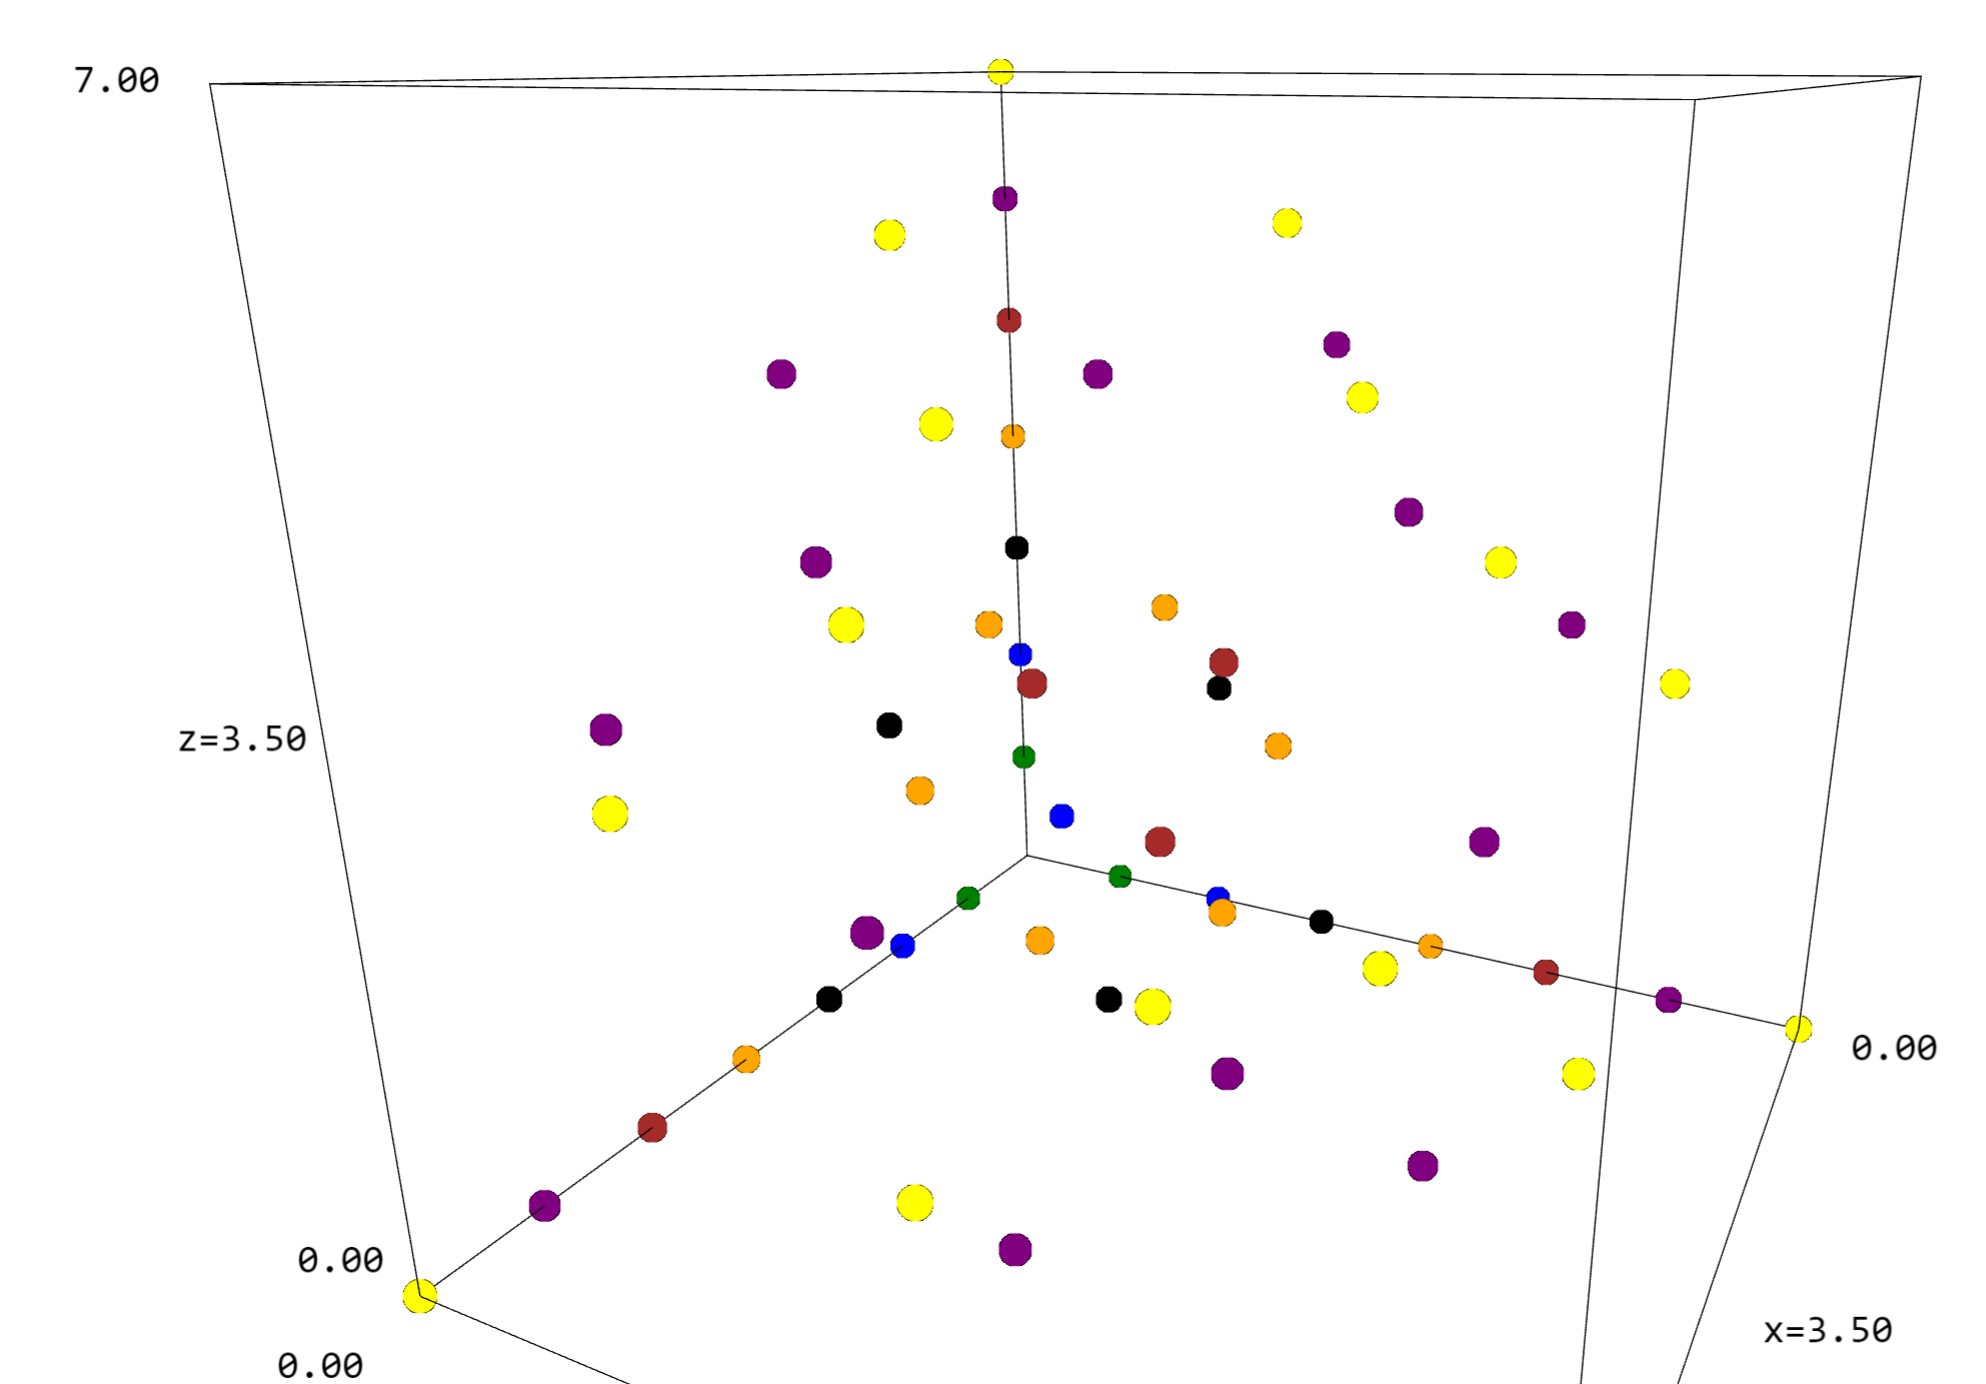
\includegraphics[height=5cm]{./img/puntos3D.png} \\
          (a) $r=2$ & (b) $r=3$  \\
        \end{tabular}
        \caption{Graphic representation of admissible $r$-indices}
        \label{fig:indices}
      \end{figure}

\section{Type I MOP in two variables}

Let us recall type I multiple orthogonal polynomials in Definition \ref{def:typeI-univar}. Given $\vec n =(n_1,\dots,n_r)$, it consists of a polynomial list $(A_{\vec n,1},\dots,A_{\vec n, r})$ where $\deg(A_{\vec n,j})\leq n_j-1$ ($j=1,\dots,r$) and polynomials $A_{\vec n,j}$ satisfy \eqref{eq:typeI-MOP} and \eqref{eq:typeI-MOP-normalization}. These two conditions can be also expresed in a more compact way if we use the inner products, see \eqref{eq:typeI-MOP-dot}.

In order to generalize this type of orthogonality, the first problem is the sum located in orthogonality condition. This forces us to define polynomials, or polynomial vectors $\mathbb A_{\vec n, j}$, of the same size. If these vectors had different size, it would not be possible to make the sum. This makes impossible to consider $\mathbb A_{\vec n,j}$ a vector of degree $\leq n_j-1$ polynomials, with size $n_j$. The solution to this problem will be explained below.

Let $\vec n = (n_1,\dots,n_r)\in\N^r$ such that the condition \eqref{eq:condition-type-ii} holds for some $n\in\N$. Then, let $i\in\{1,\dots,n\}$ and, for each $j$, the polynomial $$A_{\vec n, j}^{(i)}(x,y) = g_{n_j-1,n_j-1}^t \mathbb X_{n_j-1} + g_{n_j-1,n_j-2}^t \mathbb X_{n_j-2} + \cdots + g_{n_j-1,0}^t \mathbb X_{0}$$ with $g_{n_j-1,k}\in\R^{k+1}$ ($k=0,\dots,n_j-1$), is a bivariate polynomial such that $\deg A_{\vec n, j}^{(i)} \leq n_j-1$, ($j=1,\dots,r$). Now, given $r$ 2-dimensional measures $\mu_1,\dots,\mu_r$, we will force the polynomials $A_{\vec n, 1}^{(i)}, A_{\vec n, 2}^{(i)}, \dots, A_{\vec n, r}^{(i)}$ to satisfy the first type I multiple orthogonality condition:

\begin{equation}
    \label{eq:first-condition-type-I}
    \sum_{j=1}^r \prodesc{\mathbb X_k}{A_{\vec n,j}^{(i)}}_j = \left\{\begin{array}{ccl}
        0_{(k+1)\times 1} &   \text{ if } & k=0,\dots,n-2 \\
        (e_i)_{n\times 1} = (0,\dots,0,1,0,\dots,0)^t & \text{ if } & k=n-1      
    \end{array}\right.
\end{equation}

It is easy to see that the number of unknown coefficients of the polynomials $A_{\vec n,j}^{(i)}$ is the same as the number of linear equations given by conditions \eqref{eq:first-condition-type-I}. If we repeat this for every possible $i\in\{1,\dots,n\}$, we get $n$ lists of polynomials $A_{\vec n, j}^{(i)}$, $j=1,\dots,r, i=1,\dots,n$. Now, let us denote
$$
\mathbb A_{\vec n,j} = \begin{pmatrix}
    A_{\vec n, j}^{(1)} \\ \vdots \\ A_{\vec n, j}^{(n)}
\end{pmatrix}_{n\times 1},
$$
a polynomial vector of size $n$ whose components are bivariate polynomials of degree less than or equal to $n_j-1$ ($j=1,\dots,r$) and, fixed $i$, the polynomials $A_{\vec n, 1}^{(i)},\dots,A_{\vec n, r}^{(i)}$ satisfy \eqref{eq:first-condition-type-I}. Thus, the polynomial vectors $\mathbb A_{\vec n,j}$ will satisfy:

\begin{equation}
    \label{eq:condition-type-I}
    \sum_{j=1}^r \prodesc{\mathbb X_k}{\mathbb A_{\vec n,j}}_j = \left\{\begin{array}{ccl}
        0_{(k+1)\times n} &   \text{ if } & k=0,\dots,n-2 \\
        I_n & \text{ if } & k=n-1      
    \end{array}\right.
\end{equation}

Observe the similarity between equations \eqref{eq:typeI-MOP-function} and \eqref{eq:condition-type-I}.
    
Summarizing, we present the final definitions of the multiple orthogonal polynomials in two variables.

\begin{definition}[Type II MOP in two variables]
    Let $\vec n = (n_1, \dots, n_r)\in \N^r$ such that the condition \eqref{eq:condition-type-ii} holds for certain $n\in\N$. A vector of monic degree $n$ polynomials $\mathbb P_{\vec n}^n = \mathbb X_n + \displaystyle\sum_{k=0}^{n-1} G_{n,k} \mathbb X_k$ is a \textbf{type II Multiple Orthogonal Polynomial Vector} if 
    \begin{equation}
        \label{eq:typeII-MOP-2vars}
        \prodesc{\mathbb X_k}{\mathbb P_{\vec n}^n}_j = 0_{(k+1)\times (n+1)}, \ \ \ k=0,\dots,n_j-1, \ \ \ i=1,\dots,r
    \end{equation}      
\end{definition}

The $n+1$ bivariate polynomials composing the polynomial vector $\mathbb P_{\vec n}^n$ will be denoted as
$$
\mathbb P_{\vec n}^n = 
\begin{pmatrix}
    P_{\vec n}^{n,1}(x,y) \\ \vdots \\ P_{\vec n}^{n,n+1}(x,y)
\end{pmatrix}_{(n+1)\times 1}.
$$

\begin{definition}[Type I MOP in two variables]
    Let $\vec n = (n_1, \dots, n_r)\in \N^r$ such that the condition \eqref{eq:condition-type-ii} holds for certain $n\in\N$. \textbf{Type I Multiple Orthogonal Polynomials Vectors} are presented as $(\mathbb A_{\vec n,1}, \dots, \mathbb A_{\vec n,r})$, where 
    $\mathbb A_{\vec n,j}=(A_{\vec n,j}^{(1)}, \dots, A_{\vec n,j}^{(n)})^t$, $j=1,\dots,r$ and $A_{\vec n,j}^{(i)}$ are polynomials of degree less than or equal to $n_j-1$ for every $i=1,\dots,n$. In addition, these polynomial vectors satisfy conditions \eqref{eq:condition-type-I}.     
\end{definition}

As in the univariate case, from Type I MOP, when the 2-dimensional measures are all absolutely continuous with respect to a common positive measure $\mu$ defined in $\Omega = \displaystyle\bigcup_{j=1}^r \Omega_j$ (with $\Omega_j=\supp(\mu_j)$), \textit{i.e.}, $d\mu_j = w_j(x,y)d\mu(x,y)$, ($j=1,\dots,r$), we can define the \textit{Type I function}:
\begin{equation}
    \label{eq:type-I-function-2-vars}
    \mathbb Q_{\vec n} = \sum_{j=1}^r \mathbb A_{\vec n,j}w_j(x,y).
\end{equation}
Using this function, it is possible to rewrite \eqref{eq:condition-type-I} as

\begin{equation}
    \prodesc{\mathbb X_k}{\mathbb Q_{\vec n}}_\mu = \left\{\begin{array}{ccl}
        0_{(k+1)\times n} &   \text{ if } & k=0,\dots,n-2 \\
        I_n & \text{ if } & k=n-1.
    \end{array}\right.     
\end{equation}
We will often remove the sub-index $\mu$ from $\prodesc{\cdot}{\cdot}_\mu$, assuming that the product uses the common measure.

Despite their differences, type I and type II MOP in two variables are equivalent.
\begin{proposition}
  \label{prop:existence}
  Let $\vec n = (n_1,\dots,n_r)$ be a multi-index satisfying \eqref{eq:condition-type-ii} for $n\in\N_0$. Then the following statements are equivalent:
  \begin{enumerate}
      \item There exist unique polynomial vectors $(\mathbb A_{\vec n,1}, \dots, \mathbb A_{\vec n,r})$ of bivariate type I multiple orthogonal polynomials.
      \item There exist a unique bivariate type II multiple orthogonal polynomial $\mathbb P_{\vec n}^n$.
  \end{enumerate}
\end{proposition}

As we can see, the bivariate case reduces the number of multi-indices $(n_1,\dots,n_r)$ which it is possible to create multiple orthogonal polynomials with. Whereas in univariate case it is possible to question existence of MOP for every $\vec n\in \N^r$, in the bivariate case only some of the multi-indices can give us MOP, those such that there exist $n\in\N$ with $n(n+1)=\displaystyle\sum_{j=1}^r n_j (n_j+1)$. Given an admissible $\vec n\in\N^r$, we will say $\vec n$ is a \textbf{normal} multi-index if it satisfies the conditions of Proposition \ref{prop:existence}. A system $\mu_1,\dots,\mu_r$ of bivariate measures is \textbf{perfect} if every admissible multi-index is normal.

\section{First example}

We are going to show you the first example of type II bivariate multiple orthogonal polynomials: Multiple product Laguerre polynomials. First, we will present univariate precedents. According to \cite[Page 658, Section 3.6.1]{foupouagnigni-2020}, type II multiple Laguerre polynomials of the first kind $L_{\vec n}^{\vec\alpha}(x)$ ($\vec\alpha=(\alpha_1,\dots,\alpha_r)$) satisfy
\begin{equation}
    \int_0^\infty x^k L_{\vec n}^{\vec\alpha}(x) x^{\alpha_j} e^{-x} dx =0 \ \ \ k=0,\dots, n_j-1, \ \ j=1,\dots,r. 
\end{equation}
In order that all multi-indices to be normal we need to have $\alpha_j>-1$ and $\alpha_j- \alpha_i\not\in\Z$ whenever $i\neq j$. On the other hand, bivariate product Laguerre polynomials \cite[Ch. II, Section 2.2]{dunkl_xu_2014} are orthogonal with respect to the bidimensional weight function
$$w(x,y)=x^\alpha y^\beta e^{-x-y}, \ \ \ \alpha,\beta>-1.$$ 

Following this two approaches, we present an example with $r=3$. Let $\vec\alpha=(\alpha_1,\alpha_2,\alpha_3)$, $\vec\beta=(\beta_1,\beta_2,\beta_3)$ such that $\alpha_j,\beta_j > -1$ and any possible pair $\alpha_i,\beta_j$ satisfies $\alpha_i-\beta_j\not\in\Z$, and  $\alpha_j- \alpha_i\not\in\Z$, $\beta_j- \beta_i\not\in\Z$ whenever $i\neq j$ (any difference between different parameters is not an integer). We consider the following system of 2-dimensional measures:
\begin{align}
    d\mu_1(x,y) &= x^{\alpha_1} y^{\beta_1} e^{-x-y} d(x,y), & d\mu_2(x,y) &= x^{\alpha_2} y^{\beta_2} e^{-x-y} d(x,y),
\end{align}
$$d\mu_3(x,y) = x^{\alpha_3} y^{\beta_3} e^{-x-y} d(x,y).$$

Let $\vec n=(n_1,n_2,n_3)\in\N^3$ satisfying \eqref{eq:condition-type-ii}. Then, we have proven experimentally that many of the possible multi-indices are normal. For example, if we take $$\alpha_1 = 0, \alpha_2 = 0.5, \alpha_3 = 1.3; \beta_1 = 0.8, \beta_2 = 0.4, \beta_3 = 2.1,$$ then we can calculate the polynomial vector $\mathbb P_{(1,1,1)}^2$:
$$
\mathbb P_{(1,1,1)}^2 = \begin{pmatrix}
    x^2 + - 3.85556 x - 0.444444 y + 2.65556 \\ x y - 2.15556 x - 1.94444 y + 3.85556 \\  y^2 - 0.755556 x - 5.14444 y + 4.97556
\end{pmatrix}
$$

In the following images it is possible to see a plot of the 3 polynomials of vector $\mathbb P_{(1,1,1)}^2$ in figure \ref{fig:example} and a picture representing all three polynomials together in figure \ref{fig:example-2}.
\begin{figure}[h]
    \centering\begin{tabular}{ccc}
      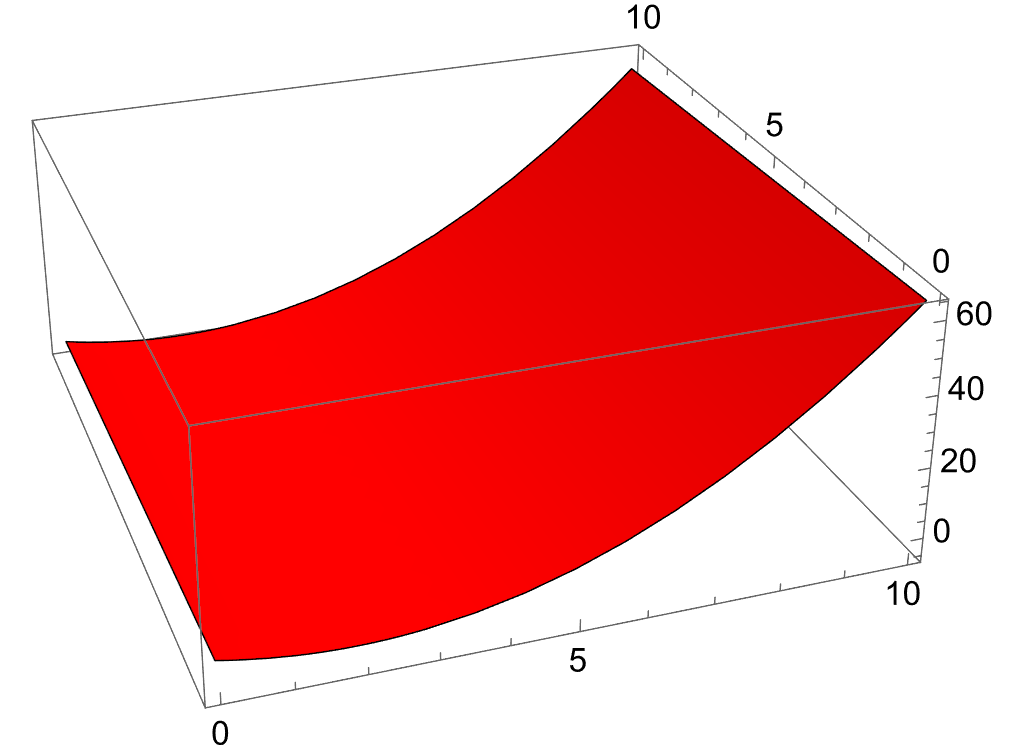
\includegraphics[width=4.5cm]{./img/laguerre1.png} & 
      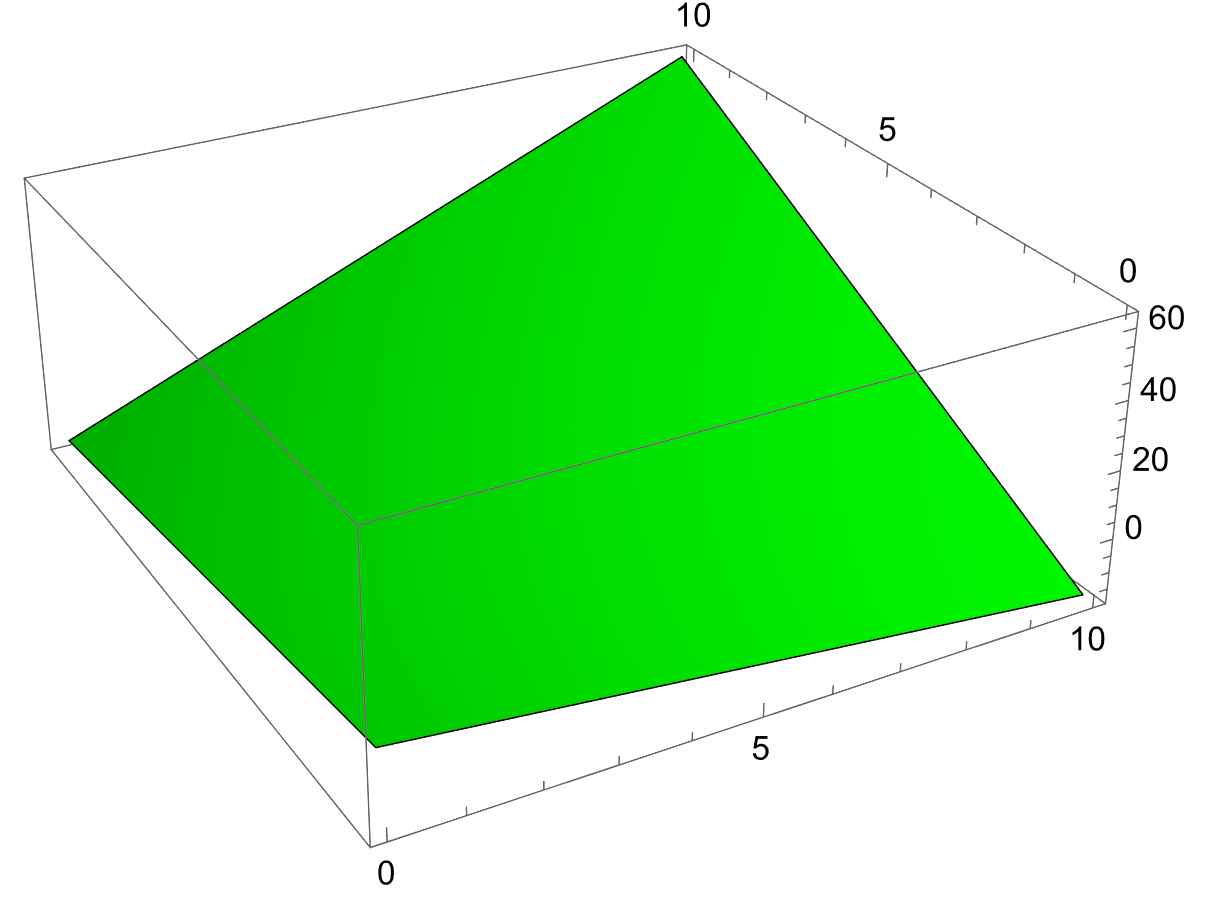
\includegraphics[width=4.5cm]{./img/laguerre2.png} &
      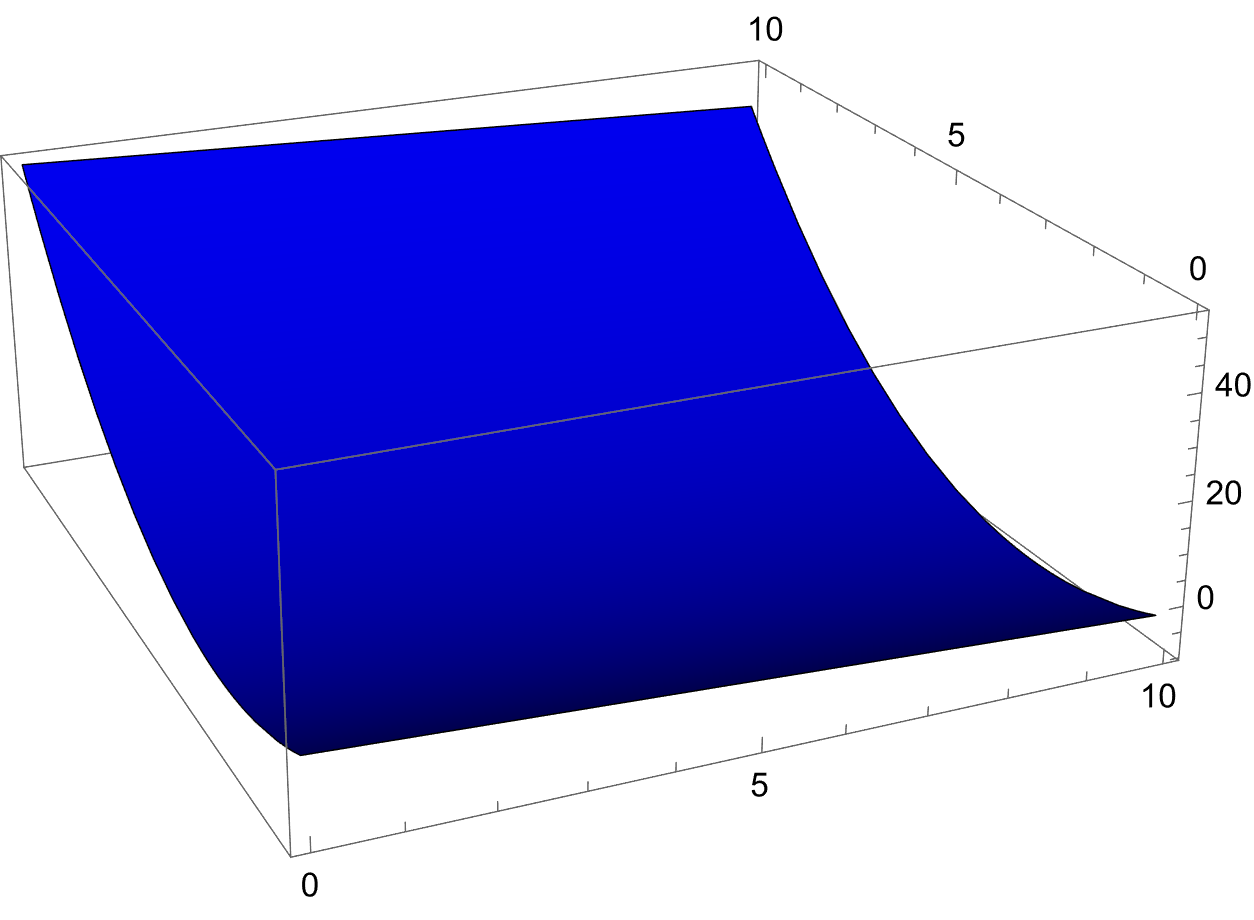
\includegraphics[width=4.5cm]{./img/laguerre3.png} \\
      (a) $(\mathbb P_{(1,1,1)}^2)_1$ & (b) $(\mathbb P_{(1,1,1)}^2)_2$ & (c) $(\mathbb P_{(1,1,1)}^2)_3$  \\
    \end{tabular}
    \caption{Graphic representation of $\mathbb P_{(1,1,1)}^2$}
    \label{fig:example}
  \end{figure}
  \begin{figure}[h]
    \centering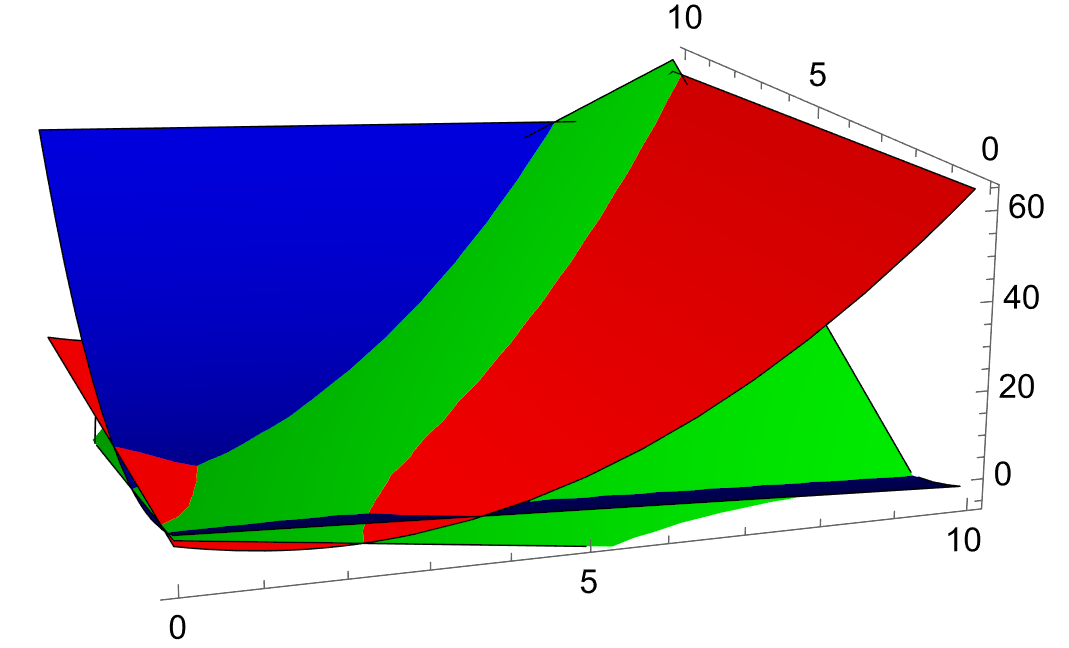
\includegraphics[width=5cm]{./img/EjemploLaguerre.png}
    \caption{$\mathbb P_{(1,1,1)}^2$ polynomials together}
    \label{fig:example-2}
  \end{figure}

  \subsection{Product of two univariate type II MOPs}

  It is well known (see \cite[Ch. II, Section 2.2]{dunkl_xu_2014}) that, given two univariate measures $\phi$ and $\psi$ and two OPS $\{P_n(x)\}$ and $\{Q_n(y)\}$ with respect to $\mu$ and $\phi$ respectively, then the polynomial vectors 
  $$
  \mathbb P_n = \left(P_n(x) Q_0(y), P_{n-1}(x)Q_1(y),\dots,P_0(x) Q_n(y)\right)^T \ \ \ \ n\geq 0
  $$
  form a system of polynomial vectors with respect to the product measure $\mu(x)\cdot \phi(y)$.
  
  Then, it seems natural to think about the product of two univariate multiple orthogonal polynomials. In this section, we will look for some bivariate multiple orthogonality relations from the product of univariate type II MOP. 
  
  First of all, let us consider two perfect measure systems $\mu_1,\dots,\mu_r$ and $\phi_1,\dots,\phi_s$ ($\Omega_j = \supp(\mu_j), \Gamma_i = \supp(\phi_i)$). Then, for every $\vec n\in \N^r, \vec m\in\N^s$, there exist $P_{\vec n}(x), Q_{\vec m}(y)$ such that
  \begin{eqnarray}
      \prodesc{P_{\vec n}(x)}{x^k}_j = \int_{\Omega_j}P_{\vec n}(x) x^k d\mu_j(x) = 0, \ \ \ \ k=0,\dots,n_j-1, \ \ j=1,\dots,r,   \\
      \prodesc{Q_{\vec m}(y)}{y^k}_i = \int_{\Gamma_i}Q_{\vec m}(y) y^k d\phi_i(y) = 0, \ \ \ \ k=0,\dots,m_i-1, \ \ i=1,\dots,s.
  \end{eqnarray}

  Then, it is possible to multiply $P_{\vec n}(x)\cdot Q_{\vec m}(y)$ and integrate both together in order to get
  \begin{equation}
    \label{eq:product-of-univariate-mop}
    \begin{split}
        \prodesc{P_{\vec n}(x)Q_{\vec m}(y)}{x^k y^t}_{j,i} &= \int_{\Omega_j}\int_{\Gamma_i} P_{\vec n}(x)Q_{\vec m}(y)x^k y^t d\mu_j(x) d\phi_i(y) \\
        &= \left(\int_{\Omega_j}P_{\vec n}(x)x^k d\mu_j(x) \right)\left(\int_{\Gamma_i} Q_{\vec m}(y) y^t  d\phi_i(y)\right) \\
        &= 0 \ \ \ 
            k = 0,\dots,n_j-1, \ \ j=1,\dots,r \text{ or } \\
        &\ \ \ \ \ \ \ \ \
            t = 0,\dots,m_i-1, \ \ i=1,\dots,s.
    \end{split}
  \end{equation}
  Now we consider the system of bidimensional measures composed of the product of every pair of one-dimensional measures $\{\mu_j\times \phi_i, \ j=1,\dots,r, \ i=1,\dots,s\}$. This set is composed of $r\cdot s$ bidimensional measures. The question now is: There exists any $v$-admissible $\vec v\in\N^{r\times s}$ such that $\mathbb P_{\vec v}^v$ is a polynomial vector whose components are product of univariate multiple orthogonal polynomials? If it exists, it is unique?

  First, we will present a lemma, which is a consecuence of the previous operations in \eqref{eq:product-of-univariate-mop}.
  \begin{lemma}
    Let $\mu_1,\dots,\mu_r$ and $\phi_1,\dots,\phi_s$ be two perfect systems of one-dimensional measures and let $\vec n\in \N^r, \vec m\in\N^s$. Let us consider $\vec v\in\N^{r\times s}$ such that $v_{ji}= \nolinebreak n_j+m_i$, $j=1,\dots,r$, $i=1,\dots,s$. Then, the bivariate polynomial $R(x,y)=P_{\vec n}(x) Q_{\vec m}(y)$ satisfies
    $$
    \prodesc{R(x,y)}{\mathbb X_k}_{j,i} = 0_{(k+1)\times 1}, \ \ \ \ k=0,\dots,v_{ji}-1, \ \  j=1,\dots,r, \ i = 1,\dots,s.
    $$
  \end{lemma}
  \begin{proof}

    Fixed $j\in\{1,\dots,r\}, i\in\{1,\dots,s\}$, the result will be proven for \linebreak $k=v_{ji}-1=n_i+m_j-1$ so that for $k\leq v_{ji}$ it would be trivially true. If $k=n_i+m_j-1$, then $\mathbb X_k = (x^k, x^{k-1}y,\dots,y^k)^T$ and its size is $k+1=n_i+m_j$. According to \eqref{eq:product-of-univariate-mop}:

    \begin{equation}
        \label{eq:lemma-1}
            \prodesc{R(x,y)}{\mathbb X_k}_{j,i} = \prodesc{P_{\vec n}Q_{\vec m} }{\mathbb X^k}_j = \begin{pmatrix}
                \prodesc{P_{\vec n}}{x^k}_j \prodesc{Q_{\vec m}}{y^0}_i \\
                \prodesc{P_{\vec n}}{x^{k-1}}_j \prodesc{Q_{\vec m}}{y^1}_i \\
                \vdots \\
                \prodesc{P_{\vec n}}{x^0}_j \prodesc{Q_{\vec m}}{y^k}_i \\
            \end{pmatrix}.
    \end{equation}

    On one hand, we know $\prodesc{Q_{\vec m}}{y^l}_i =0$ whenever $0\leq l \leq m_i-1$, so that the first $m_i$ components of the vector are $0$. On the other hand $\prodesc{P_{\vec n}}{x^{k-l}}_j =0$ whenever $0\leq k-l \leq n_j-1$, so that the last $n_j$ components are also $0$. As its size is $k+1=n_i+m_j$, then the vector in \eqref{eq:lemma-1} is equal to $0_{(k+1)\times 0}$.

  \end{proof}

  \cred{REVIEW No me convence lo del $j,i$ cuando se suele poner $i,j$, pero es porque incialmente siempre hemos empezado a numerar las medidas con la $j$ y cuando hemos metido el segundo conjunto de medidas las hemos numerado con la $i$.}

  At this moment, we know $R(x,y)$ satisfies orthogonality relations with respect to $\tilde v = \left(\tilde v_{ji} = n_j + m_i, j=1,\dots,r, \ i=1,\dots,s \right)$ and the system of bidimensional measures $\{\mu_j \times \phi_i, \ j=1,\dots,r, \ i=1,\dots,s\}$. Now, our question is, there exists any $v$-admissible multi-index $v\in \N^{r\times s}$ such that $v_{ji}\leq \tilde v_{ji}$ (so that the orthogonality relations still hold) for every possible $\vec n\in \N^r$ and $\vec m\in \N^s$? And if it exists, is there any relation between $P_{\vec v}^v$ and the polynomials $P_{\vec n}, Q_{\vec m}$?

  In order to check this conjecture, we asked ourselves if 
  $$
  \sum_{j=1}^r \sum_{i=1}^s \tilde v_{ji}(\tilde v_{ji}+1) \geq (|\vec n|+|\vec m|) (|\vec n|+|\vec m|+1).
  $$
  If this inequality was true for every possible $\vec n,\vec m$, then we could ensure that it is always possible to find a $v$-admissible multi-index $v\in \N^{r\times s}$ such that $v_{ji}\leq \tilde v_{ji}$. However, we found several examples contradicting this hypotesis:

  If $r=4$ and $s=2$, let us consider $\vec n = (3,3,4,1)$ and $\vec m = (0,1)$. Then $\tilde{v} = (3,4,3,4,4,5,1,2)$, with $$\sum_{l=0}^{8}\tilde v_l (\tilde v_l+1) = 122 \not\geq 156 = (12\cdot 13) = (|\vec n|+|\vec m|) (|\vec n|+|\vec m|+1).$$

  This was one of the reasons why we decided to try a different way of generalizing to the bivariate case the multiple  (see chapter \ref{chap:II}). But, before that, we were able to extend two important results, which are written below.



\section{Biorthogonality}

Let $\mu_1,\dots,\mu_r$ be a perfect system of $r$ 2-dimensional measures. In this section, we will explain an orthogonality relation between type I and type II MOP. Analogous results for the univariate case are available in \cite[Theorem 23.1.6]{Ismail}.

\begin{theorem}
    \label{th:biorthogonality}
    Given $\vec n, \vec m$, both satisfying \eqref{eq:condition-type-ii} for $n$ and $m$, respectively, the following biorthogonality holds for type I and type II MOP:
    \begin{equation}
        \prodesc{\mathbb P_{\vec n}^n}{\mathbb Q_{\vec m}} = \left\{\begin{array}{ccl}
            0_{(n+1)\times m} &   \text{ if } & \vec m \leq \vec n \\
            0_{(n+1)\times m} &   \text{ if } &  n \leq m -2 \\
            I_{n+1} & \text{ if } & n=m-1 
        \end{array}\right.   
    \end{equation}
\end{theorem}
\begin{proof}
    We will prove each item. First, we have
    \begin{equation*}
        \prodesc{\mathbb P_{\vec n}^n}{\mathbb Q_{\vec m}} = \sum_{j=1}^r \prodesc{\mathbb{P}_{\vec n}^n}{\mathbb A_{\vec m, j}}_j.
    \end{equation*}
    \begin{itemize}
        \item Assume $\vec m \leq \vec n$, this means $m_j \leq n_j \ \ \forall j\in\{1,\dots,r\}$. Then, remember $\mathbb{A}_{\vec m,j}$ is a vector of polynomials of degree less than or equal to $m_j-1 < n_j$ for every $j\in\{1,\dots,r\}$ and $\prodesc{\mathbb P_{\vec n}^n}{\mathbb Q_{\vec m}} =0$ follows from type II orthogonality conditions \eqref{eq:typeII-MOP-2vars}.
        \item  If $n\leq m-2$, then each polynomial of $\mathbb P_{\vec n}^n$ is a linear combination of $\mathbb X_{n-2},\dots,\mathbb X_1,\mathbb X_0$. Then, type I orthogonality conditions \eqref{eq:condition-type-I} for $0\leq k\leq n-2$ shows $\prodesc{\mathbb P_{\vec n}^n}{\mathbb Q_{\vec m}} =0$.
        \item Finally, if $m=n+1$, then $\mathbb P_{\vec n}^n$ is a vector of degree $m-1$ polynomials. So, $\mathbb P_{\vec n}^n = \mathbb X_{m-1} + \displaystyle\sum_{k=0}^{m-2} G_{k} \mathbb X_{k}$. Due to the previous item, we have
        $$
        \prodesc{\mathbb P_{\vec n}^{m-1}}{\mathbb Q_{\vec m}} = \sum_{j=1}^r \prodesc{\mathbb{P}_{\vec n}^{m-1}}{\mathbb A_{\vec m, j}}_j = \sum_{j=1}^r \prodesc{\mathbb X_{m-1}}{\mathbb A_{\vec m, j}}_j = I_m = I_{n+1},
        $$
        where in the second last equality we have used the normalization condition in \eqref{eq:condition-type-I}.
    \end{itemize}
\end{proof}

Observe that the first item emphasises the components of multi-indices $\vec n$ and $\vec m$, while the last two items are true for any two multi-indices with degree $n$ and $m$ whatever their components are.

This result, which is a two-dimensional extension of \cite[Theorem 23.1.6]{Ismail}, will be very useful in order to prove the next result.


\section{Nearest Neighbour Recurrence Relation}
\label{sec:NNRR}

The standard orthogonal polynomials always satisfy a Three-Term Recurrence Relation. That is, given an monic OPS $\{P_n\}$ with respect to a inner product $\prodesc{\cdot}{\cdot}$ or its respective functional $\mathcal L$, there exist constants $\alpha_n,\beta_n$ such that
$$
xP_n = P_{n+1}+ \alpha_n P_n + \beta_n P_{n-1}.
$$
The nearest Neighbour Recurrence Relation, in univariate multiple orthogonality, extends this result, allowing us to express a type II polynomial multiplied by $x$: $xP_{\vec n}$ as a linear combination of the polynomial itself, $P_{\vec n}$, a beyond neighbour, \textit{i.e.} $P_{\vec n + e_k}$ and $r$ above neighbours, see \cite[Theorem 23.1.7]{Ismail}. We are going to give a proof of a first generalization to bivariate MOP of this result. 

\begin{theorem} 
    \label{th:neighbours}
    Let $\mu_1,\dots,\mu_r$ be a perfect system of 2-dimensional measures. Let $\vec n\in \N^r$ be a multi-index satisfying \eqref{eq:condition-type-ii} for $n\in\N$ and let us consider a path $\{\overrightarrow{m}_k:k=0,\dots,n+1\}$ where $\overrightarrow{m}_0=\vec 0, \overrightarrow{m}_n = \vec n$, each $\overrightarrow{m}_k$ satisfy \eqref{eq:condition-type-ii} for $k$ and $\overrightarrow{m}_k \leq \overrightarrow m_{k+1}$ for $k=0,\dots,n$. Then, there exist matrices $A_0,\dots,A_r$ of sizes $(n+1)\times(n-j+1)$,  $(j=0,\dots,r)$ such that
    \begin{equation}
        \label{eq:nearest-neighbour}
        x\mathbb P_{\vec n}^n = L_{{n+1},1} \mathbb P_{\overrightarrow{m}_{n+1}}^{n+1} + A_0 \mathbb P_{\vec n}^n + \sum_{j=1}^r A_j \mathbb P_{\overrightarrow{m}_{n-j}}^{n-j},
    \end{equation}
    where $L_{n+1,1}=(I_{n+1}|0_{(n+1)\times 1})$.

    In addition, $A_j = \prodesc{x\mathbb P_{\vec n}^n}{\mathbb Q_{\overrightarrow{m}_{n-j+1}}}$.
\end{theorem}
\begin{proof}
    As we are in a perfect system, we can assume the existence of $\mathbb P_{\overrightarrow{m}_k}^k$ for every $\vec m_k, k=0,\dots,n+1$. As we know, $x\mathbb P_{\vec n}^n$ is a vector of degree $n+1$ polynomials and its size is also $n+1$. It is possible to write  $x\mathbb P_{\vec n}^n$ as a linear combination of $\{\mathbb P_{\overrightarrow{m}_k}^k, k=0,\dots,n+1\}$ whose coefficients are matrices $M_k$:
    $$
    x\mathbb P_{\overrightarrow{n}}^n = \sum_{k=0}^{n+1} M_k \mathbb P_{\overrightarrow{m}_k}^k,
    $$
    where $M_k$ is a $(n+1)\times(k+1)$ matrix ($k=0,\dots,n+1$).

    Observing the leader term of $x\mathbb P_{\overrightarrow{n}}^n$, which is $x\mathbb X_{n}$, and comparing it with the leader term of $M_{n+1} \mathbb P_{\overrightarrow{m}_{n+1}}^{n+1}$, which is $M_{n+1}\mathbb X_{n+1}$ we can easily check $M_{n+1}=L_{(n+1),1}$. Now, we have
    $$
    \mathbb P_{\overrightarrow{n}}^n = L_{n+1,1}\mathbb P_{\overrightarrow{m}_{n+1}}^{n+1} + \sum_{k=0}^{n} M_k \mathbb P_{\overrightarrow{m_k}}^k.
    $$
    Now, we apply the inner product to both sides of the equation by $\mathbb Q_{\overrightarrow{m}_l}$ and observe:
    \begin{itemize}
        \item If $\overrightarrow{m}_l\leq \overrightarrow{m}_j$, which always happens if $l\leq j\leq n+1$, then, due to the first item of Theorem \ref{th:biorthogonality}, $\prodesc{\mathbb P_{\overrightarrow{m}_j}^j}{\mathbb Q_{\overrightarrow{m}_l}} = 0_{(j+1)\times l}$ whenever $l\leq j$.
        \item If $j\leq l-2$, then, from the second item of Theorem \ref{th:biorthogonality}, $\prodesc{\mathbb P_{\overrightarrow{m}_j}^j}{\mathbb Q_{\overrightarrow{m}_l}} = 0_{(j+1)\times l}.$
        \item Finally, if $j=l-1$, from the last item of Theorem \ref{th:biorthogonality} we deduce $\prodesc{\mathbb P_{\overrightarrow{m}_j}^j}{\mathbb Q_{\overrightarrow{m}_l}} = I_{j+1}.$
    \end{itemize}

    Summarizing, we have
    $$
    \prodesc{x\mathbb P_{\vec n}^n}{\mathbb Q_{\overrightarrow{m}_l}} = L_{n+1,1}\prodesc{\mathbb P_{\overrightarrow{m}_{n+1}}^{n+1}}{\mathbb Q_{\overrightarrow{m}_l}} + \sum_{j=0}^n M_j \prodesc{\mathbb P_{\overrightarrow{m}_j}^j}{\mathbb Q_{\overrightarrow{m}_l}}.
    $$
    Applying the previous items deduced from Theorem \ref{th:biorthogonality}, we have
    \begin{equation}
        \label{eq:biorthogonality-1}
        \prodesc{x\mathbb P_{\vec n}^n}{\mathbb Q_{\overrightarrow{m}_l}} = M_{l-1} \ \ \ \ l=1,\dots,n+1,
    \end{equation}

    Now, if $l\leq n-r$, then $\overrightarrow{m}_l\leq \overrightarrow{m}_{n-r}$. So, choosing $l\leq n-r$,
    $$
    \prodesc{x\mathbb P_{\vec n}^n}{\mathbb Q_{\overrightarrow{m}_l}} = \sum_{j=1}^r  \prodesc{\mathbb P_{\vec n}^n}{x\mathbb A_{\overrightarrow{m}_l,j}}_j,
    $$
    but $x\mathbb A_{\overrightarrow{m}_l,j}$ are vectors of degree less than or equal to $(\overrightarrow{m}_l)_j\leq (\overrightarrow{m}_{n-r})_j < n_j$. Then, the product vanishes because of type II orthogonality \eqref{eq:typeII-MOP-2vars}. This means
    $$
    \prodesc{x\mathbb P_{\vec n}^n}{\mathbb Q_{\overrightarrow{m}_l}} = M_{l-1} = 0 \ \ \ l = 1, \dots, n-r.
    $$
    Thus, the final expression is
    $$
    \mathbb P_{\overrightarrow{n}}^n = L_{n+1,1}\mathbb P_{\overrightarrow{m}_{n+1}}^{n+1} + \sum_{k=n-r}^{n} M_k \mathbb P_{\overrightarrow{m}_k}^k.
    $$
    If we rename $A_{n-k} = M_k$ for $k=n-r,...,n$, then we get the desired expression \eqref{eq:nearest-neighbour}. 

    Finally, due to \eqref{eq:biorthogonality-1}, $$A_j = M_{n-j} =  \prodesc{x\mathbb P_{\vec n}^n}{\mathbb Q_{\overrightarrow{m}_{n-j+1}}}.$$
\end{proof}

Nevertheless, this theorem has a significant limitation: There are admissible multi-index $\vec n$ such that it is not possible to build a path from $\vec 0$ to $\vec n$ with exactly $n$ steps. For example, when $r=3$, the multi-index $\vec n =(1,4,4)$ satisfy condition \eqref{eq:condition-type-ii} for $n=6$. However, looking at table \ref{tab:3measuresindices} it is clear that there is not any multi-index $\vec m$ with degree 5 and $\vec m \leq \vec n$. 

In fact, this problem holds when the polynomials' degree or the number of measures $r$ increase. For example, when $r=5$, $(1,4,4,0,0)$ (degree 6), $(5,6,0,0,0)$ (degree 8) or $(1,1,1,6,6)$ (degree 9) have not any possible path from $\vec 0$ satisfying theorem \ref{th:neighbours}.


\chapter{Second approach: Using the Graded Reverse Lexicographic Order}
\label{chap:II}

The second way we tried to generalize multiple orthogonality to the bivariate case was by using the basis of bivariate polynomials ordered by the graded reverse lexicographic order, this is
\begin{equation}
    \label{eq:usual-basis-ordered}
    \{1,x,y,x^2,xy,y^2,x^3,x^2y,xy^2,y^3,\dots\}
\end{equation}
On the other hand, it is known $\N$ and $\N^2$ are isomorphic sets, so we will use the \emph{Cantor Pairing Function} $\pi$, which is a bijection between $\N$ and $\N^2$ (see \cite{Lisi}). Its expression is given by 
$$
\pi(k_1, k_2) = \dfrac{1}{2}(k_1 + k_2)(k_1 + k_2 + 1) + k_2.
$$
In figure  \ref{fig:Cantor} you can observe a graphic representation of this bijection.

\begin{figure}[h]
    \centering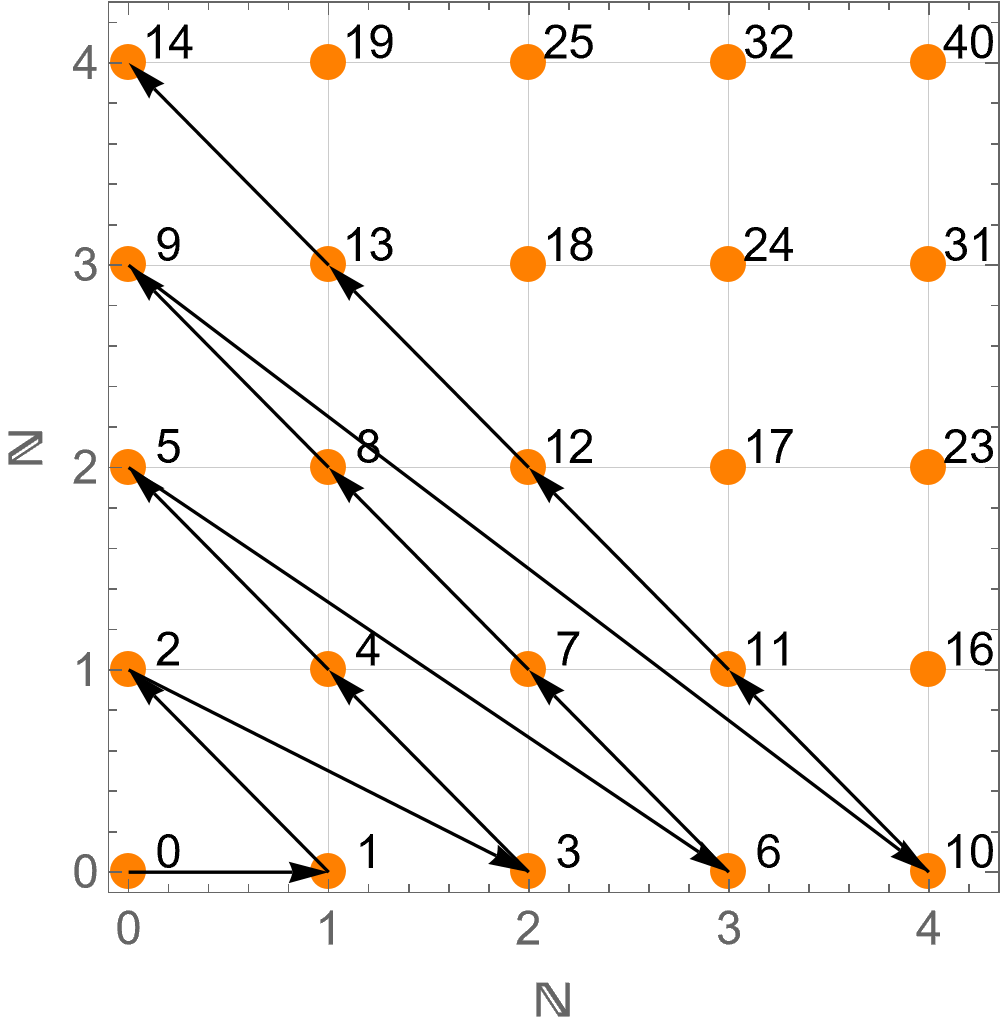
\includegraphics[width=5cm]{./img/Cantor.png}
    \caption{Graphic representation of Cantor Pairing Function}
    \label{fig:Cantor}
  \end{figure}

Starting from this, we tried to do a generalization of univariate multiple orthogonality where $|\vec n| = \pi(\exp(P_{\vec n}))$, instead of the degree of type II polynomial, where the function ``$\exp$'' represents the exponent of a polynomial (not the exponential function), \textit{i.e.}, if $$P(x,y)= c_{k} x^t y^s + c_{k-1} x^{t+1} y^{s-1} + \cdots c_2 y + c_1 x + c_0,$$ then $\exp(P)=(t,s)$ and $\pi(t,s)=k$. %Given $(k_1,k_2)\in\N^2$, we will use the notation $X^{(k_1,k_2)}:=x^{k_1} y^{k_2}$, and, if $k=\pi(k_1,k_2)$, then $X^{\pi^{-1} (k)}=X^{(k_1,k_2)}=x^{k_1} y^{k_2}$. 

Now, given $r\in\N$, $\vec n = (n_1,\dots, n_r)\in\N^r$ and a system of $r$ $2$-dimensional measures $\mu_1, \dots, \mu_r$, we are now presenting the definitions of type I and II multiple orthogonality following this approach. 

\begin{definition}[Type II Multiple Orthogonality]
  The \textbf{bivariate type II multiple orthogonal polynomial} $P_{\vec n}(x,y)$ is a monic polynomial such that $\exp(P_{\vec n})=\pi^{-1}(|\vec n|)$. This means that, if $|\vec n|=\pi(k,l)$ then 
  $$
    P_{\vec n}(x,y) = x^k y^l + c_{|\vec n|-1} x^{k+1} y^{l-1} + \cdots + c_1 x + c_0
  $$
  satisfying
  \begin{equation}
    \label{eq:typeII-MOP-2-app}
    \prodesc{P_{\vec n}}{x^t y^s}_j = 0, \ \ \ 0\leq \pi(t,s)\leq n_j-1, \ j=1,\dots,r.
  \end{equation}    
\end{definition}

In order to calculate the $|\vec n|$ coefficients of the polynomial $P_{\vec n}(x,y)$, employing the conditions \eqref{eq:typeII-MOP-2-app} we deduce the coefficients $c_0,\dots,c_{|\vec n|-1}$ are the solutions of the following system of linear equations.

\begin{equation}
    \label{eq:system-typeII-2app}
    \begin{pmatrix}
        m_{0,0}^{(1)} & m_{(1,0)}^{(1)} & \cdots &  m_{\pi^{-1}(|\vec n|-1)}^{(1)} \\
        \vdots & \vdots & \ddots & \vdots  \\
        m_{\pi^{-1}(n_1-1)}^{(1)} & m_{(1,0)+\pi^{-1}(n_1-1)}^{(1)} & \cdots &  m_{\pi^{-1}(|\vec n|-1)+\pi^{-1}(n_1-1)}^{(1)} \\ \hline
        \vdots & \vdots & \ddots  & \vdots \\ \hline
        m_{0,0}^{(r)} & m_{(1,0)}^{(r)} & \cdots  & m_{\pi^{-1}(|\vec n|-1)}^{(r)} \\
        \vdots & \vdots & \ddots & \vdots \\
        m_{\pi^{-1}(n_r-1)}^{(r)} & m_{(1,0)+\pi^{-1}(n_r-1)}^{(r)} & \cdots  & m_{\pi^{-1}(|\vec n|-1)+\pi^{-1}(n_r-1)}^{(r)}
    \end{pmatrix}\begin{pmatrix}
        c_0 \\ c_1 \\ \vdots \\ c_{|\vec n|-1}
    \end{pmatrix} = - \begin{pmatrix}
        m_{\pi^{-1}(|\vec n|)}^{(1)} \\ m_{\pi^{-1}(|\vec n|)+(1,0)}^{(1)} \\ \vdots \\ m_{\pi^{-1}(|\vec n|)+\pi^{-1}(n_1-1)}^{(1)} \\ \hline \vdots \\ \hline \\ m_{\pi^{-1}(|\vec n|)}^{(r)} \\ m_{\pi^{-1}(|\vec n|)+(1,0)}^{(r)} \\ \vdots \\ m_{\pi^{-1}(|\vec n|)+\pi^{-1}(n_r-1)}^{(r)} 
    \end{pmatrix}.
\end{equation}

We will denote as $M_{\vec n}$ the transpose matrix of the coefficients matrix of the system \eqref{eq:system-typeII-2app}. Thus, given a multi-index $\vec n =(n_1,\dots,n_r)$, the type II polynomial $P_{\vec n}$ will exist and be unique if, and only if, the matrix $M_{\vec n}$ is regular. Once the type II bivariate multiple orthogonality has been defined, we are presenting a definition for the type I MOP.

\begin{definition}[Type I Multiple Orthogonality]
  \textbf{Bivariate type I multiple orthogonal polynomials} are presented in a vector $(A_{\vec n,1}(x,y),\dots,A_{\vec n,r}(x,y))$ where $\pi(\exp(A_{\vec n,j})) \leq n_j-1$. This means, if $n_j-1 = \pi(k_j,l_j)$, then $$A_{\vec n,j} = c_{n_j-1,j} x^{k_j}y^{l_j}+ c_{n_j-2,j}x^{k_j+1}y^{l_j-1} +\cdots +c_{1,j} x + c_{0,j}$$. This polynomials satisfy
  \begin{equation}
    \label{eq:condition-type-I-2-app}
    \sum_{j=1}^r \prodesc{A_{\vec n,j}}{x^t y^s}_j = \left\{\begin{array}{ccl}
        0 &   \text{ if } & 0\leq \pi(t,s)\leq |\vec n|-2 \\
        1 & \text{ if } & \pi(t,s)= |\vec n|-1     
    \end{array}\right..
  \end{equation}
\end{definition}

Once again, let us assume the measures $\mu_1,\dots,\mu_r$ to be absolutely continuous with respect to a common measure $\mu$ whose support is $\Omega = \displaystyle\bigcup_{j=1}^r \Omega_j$, where $\Omega_j=\supp(\mu_j)$ (this is, $d\mu_j(x,y)=w_j(x,y)d\mu(x,y), \ j=1,\dots,r$). Then, we define the \textit{Bivariate Type I Function} as
\begin{equation}
    \label{eq:typeI-function-2-app}
    Q_{\vec n}(x,y)=\sum_{j=1}^r A_{\vec n,j}(x,y) w_j(x,y),
\end{equation}
so that conditions \eqref{eq:condition-type-I-2-app} are equivalent to
\begin{equation}
    \label{wq:typeI-conditions-function-2-app}
    \prodesc{Q_{\vec n}}{x^t y^s}_\mu = \left\{\begin{array}{ccl}
        0 &   \text{ if } & 0\leq \pi(t,s)\leq |\vec n|-2 \\
        1 & \text{ if } & \pi(t,s)= |\vec n|-1     
    \end{array}\right..
\end{equation}

As we have done previously, we can apply conditions \eqref{eq:condition-type-I-2-app} to generic polynomials to obtain the system of equations for the coefficients of type I polynomials $A_{\vec n,1}(x,y),\dots,A_{\vec n, r}(x,y)$. Then, type I polynomials coefficients $c_{0,j},\dots c_{n_1-1,j}, \ (j=1,\dots,r)$ are the solutions of the system 

\begin{equation}
    \label{eq:system-typeI-2app}
    M_{\vec n} \begin{pmatrix}
        c_{0,1} \\ \vdots \\ c_{n_1-1,1} \\ \hline \vdots \\ \hline c_{0,r} \\ \vdots \\ c_{n_r-1,r} 
    \end{pmatrix} = \begin{pmatrix}
        0 \\ 0 \\ \vdots \\ 0 \\ 1
    \end{pmatrix} 
\end{equation}

Observe the fact that the coefficient matrices of systems \eqref{eq:system-typeII-2app} and \eqref{eq:system-typeI-2app} are mutually transposed. As a result, the existences of type I and type II MOP for a multi-index $\vec n\in\N^r$ are equivalent. We have proven

\begin{proposition}
    \label{prop:equivalence-2-app}
    Given $\vec n=(n_1,\dots,n_r)\in\N^r$. Then the following statements are equivalent.
    \begin{enumerate}
        \item There exist unique type I polynomials $A_{\vec n,1},\dots,A_{\vec n,r}$.
        \item There exist an unique type II polynomial $P_{\vec n}$.
        \item The matrix
            \begin{equation}
                M_{\vec n} = \begin{pmatrix}
                    M^{(1)} | \cdots | M^{(r)}
                   \end{pmatrix},
            \end{equation} 
            where
            \begin{equation}
                M^{(j)} = \begin{pmatrix}
                    m_{0,0}^{(j)} & \cdots & m_{\pi^{-1}(n_j-2)}^{(j)}  & m_{\pi^{-1}(n_j-1)}^{(j)}  \\
                    m_{1,0}^{(j)} & \cdots & m_{\pi^{-1}(n_j-2)+(1,0)}^{(j)}  & m_{\pi^{-1}(n_j-1)+(1,0)}^{(j)}  \\
                    \vdots & \ddots & \vdots & \vdots \\
                    m_{\pi^{-1}(|\vec n|-1)}^{(j)} & \cdots & m_{\pi^{-1}(n_j-2)+\pi^{-1}(|\vec n|-1)}^{(j)}  & m_{\pi^{-1}(n_j-1)+\pi^{-1}(|\vec n|-1)}^{(j)}  \\
                  \end{pmatrix}
            \end{equation}
            is regular.
    \end{enumerate}
\end{proposition}

  As a consecuence of this last result, given a system of $r$ bidimensional measures $\mu_1,\dots,m_r$ and a multi-index $\vec n=(n_1,\dots,n_r)\in\N^r$, we will say $\vec n$ is \textbf{normal} if proposition \ref{prop:equivalence-2-app} holds, and the system of measures $\mu_1,\dots,\mu_r$ will be a \textbf{perfect} system of measures if every multi-index $\vec n\in\N^r$ is normal. 
  
  Comparing this latest approach with the first one, note that with the first approach only a few multi-indices allowed us to create MOP vectors, whereas in this second approach it is possible to calculate bivariate MOP with any $\vec n\in\N^r$. Apart from that, the exponent of type II polynomials is $\pi^{-1}(|\vec n|)$ and the number of orthogonality conditions in type I orthogonality is exactly $|\vec n|$, just like happens in univariate multiple orthogonality. Nevertheless, the conditions \eqref{eq:typeII-MOP-2-app} and \eqref{eq:condition-type-I-2-app} are less intuitive than \eqref{eq:typeII-MOP-d-variables} and \eqref{eq:condition-type-I} with respect to original conditions \eqref{eq:typeII-MOP-dot} and \eqref{eq:typeI-MOP-dot}.

    In the following sections, some other generalizations to the principal univariate results will be given, including a biorthogonality relation, the nearest neighbour relation and some conclusions about the product of univariate multiple orthogonal polynomials.


    \section{Biorthogonality}

    Employing the type I function defined in \eqref{eq:typeI-function-2-app} we are able to proof some orthogonality relations between type I and type II multiple orthogonal polynomials, as happened in the univariate case (see \cite[Theorem 23.1.6]{Ismail}) and also in the first approach (theorem \ref{th:biorthogonality}). 

    \begin{theorem}
        \label{th:biorthogonality-2-app}
        Let $\mu_1,\dots,\mu_r$ be a perfect system of bivariate absolutely continuous measures and consider $\vec n,\vec m\in\N^r$. Then, the following biorthogonality relation holds:
        \begin{equation}
            \label{eq:biorthogonality-2-app}
            \prodesc{P_{\vec n}}{Q_{\vec m}}_{\mu} = \left\{\begin{array}{ccc}
                0 & \text{ if } & \vec m \leq \vec n \\
                0 & \text{ if } & |\vec n| \leq |\vec m|-2 \\
                1 & \text{ if } & |\vec n| = |\vec m|-1 
            \end{array}\right.
        \end{equation}
    \end{theorem}
    \begin{proof}
        Applying the definition of type I function $Q_{\vec m}$ in \eqref{eq:typeI-function-2-app}, $$\prodesc{P_{\vec n}}{Q_{\vec m}}_{\mu} =\displaystyle\sum_{j=1}^r \prodesc{P_{\vec n}}{A_{\vec m,j}}_j.$$
        \begin{itemize}
            \item If $\vec m \leq \vec n$ (using the product order), then $m_j\leq n_j$ for every $j$. As we know $\pi(\exp(A_{\vec m,j}))\leq m_j-1 \leq n_j -1$, due to type II orthogonality $\prodesc{P_{\vec n}}{A_{\vec m,j}}_j=0$ for every $j$.
            \item If $|\vec n|\leq|\vec m|-2$, then $|\vec n|=\pi(\exp(P_{\vec n}))\leq|\vec m|-2$, so that $\displaystyle\sum_{j=1}^r\prodesc{P_{\vec n}}{A_{\vec m,j}}_j = 0$ because of type I MOP.
            \item If $|\vec n|=|\vec m|-1$, then  $|\vec n|=\pi(\exp(P_{\vec n}))=|\vec m|-1$ and, again due to type I MOP and the fact of $P_{\vec n}$ is a monic polynomial, $\displaystyle\sum_{j=1}^r\prodesc{P_{\vec n}}{A_{\vec m,j}}_j = 1$.
        \end{itemize}
    \end{proof}

    \section{Nearest Neighbour Recurrence Relation}

    Given $\vec n\in\N^r$, the original univariate Nearest Neighbour Relation \cite[Theorem 23.1.7]{Ismail} expresses the polynomial $xP_{\vec n}(x)$ as a linear combination of $P_{\vec n}$ itself, a beyond neighbour and $r$ above neighbours. In the bivariate case, we could do a generalization of this result using polynomial vectors (check section \ref{sec:NNRR}). The main problem of this result was the restrictions found in creating paths from $\vec 0$ to $\vec n$. With this approach, it is possible to solve that problem, although some other ones appeared.
    
    Firstly, in the univariate case, it is clear that $\deg(x P_{\vec n})=\deg(P_{\vec n})+1=|\vec n|+1$, and that is the reason why only one beyond neighbour is needed. However, this equality does not hold in the bivariate case with this approach. For this reason, we present de following lemma.
    
    \begin{lemma}
        \label{lemma:pi-xPn}
        Let $\vec n\in\N^r$ and $(t,s)=\exp(P_{\vec n})=\pi^{-1}(k)$. Then, $$(t+1,s)=\exp(xP_{\vec n})=\pi^{-1}(k+\deg(P_{\vec n})+1).$$
    \end{lemma}
    \begin{proof}
        Remember the usual basis of the vector space of bivariate polynomials ordered by the reverse lexicographic graded order
        $$
        \{1,x,y,\dots, x^{t+s},\dots, \underbrace{x^t y^s, x^{t-1}y^{s+1}, \dots, x y^{t+s-1},y^{t+s},x^{t+s+1},\dots,x^{t+1}y^s},\dots\}.
        $$
        An alternative interpretation of the function $\pi(t,s)$ is the position of the monomial $x^t y^s$ on this list (starting the count in $0$). In this way, $t+s+1$ monomials separate $x^t y^s$ and $x^{t+1} y^s$. Thus, $\pi(t+1,s)=\pi(t,s)+t+s+1 = k + \deg(P_{\vec n}) +1$. 
    \end{proof}

    Another useful result which will be needed is the one who expresses the degree of a  $x^t y^s$ such that we only know $k=\pi(t,s)$, but the exponent $(t,s)$ is unknown. This is, we need to calculate the degree of the $k+1$ monomial in the list \eqref{eq:usual-basis-ordered}.

    \begin{lemma}
        \label{lemma:degree}
        Let $k \in \N\cup\{0\}$ and $(t,s)=\pi^{-1}(k)$. Then 
        \begin{equation}
        t+s =\deg(x^t y^s)= \left\lceil \dfrac{1}{2}(-1+\sqrt{9+8k}) \right\rceil-1.
        \end{equation}
    \end{lemma}
    \begin{proof}
        We know there is $1$ monomial of degree $0$ ($1$), $2$ monomials of degree $1$ ($x, y$), \dots, $n+1$ monomials of degree $n$ ($x^n, x^{n-1}y, \dots, y^n$). Then, making partial sums, there are $1+2+\cdots + n+1=\dfrac{1}{2}(n+2)(n+1)$ monomials with degree $\leq n$. So, the question is, which is the minimun $n\in\N\cup\{0\}$ s.t. $\dfrac{1}{2}(n+2)(n+1)\geq k+1$?

        If we solve the last inequation, which is equivalent to $n^2 + 3n -2k \geq 0$, considering that $n\geq 0$, we get $n\geq \frac 1 2 (-3+\sqrt{9+8k})$. But $n$ has to be an integer, so we take 
        $$
        n=  \left\lceil\frac 1 2 (-3+\sqrt{9+8k})\right\rceil = \left\lceil\frac 1 2 (-1+\sqrt{9+8k})\right\rceil -1.
        $$

    \end{proof}

    With these two previous lemmas, we are able to announce the main theorem of this section

    \begin{theorem}
        Let $(\mu_1,\dots,\mu_r)$ be a perfect system of bidimensional measures and $\vec n\in\N^r$ s.t. $(t,s)=\pi^{-1}(|\vec n|)$ with $s\neq 0$. Let us consider $\vec m$ s.t. $|\vec m| = \pi(t+1,s)$ and a path $\{\vec m_k, k=0,\dots,|\vec n|,\dots,|\vec m|\}$ with $\vec m_0=\vec 0$, $\vec m_{|\vec n|}=\vec n$, $\vec m_{|\vec m|}=\vec m$ and $|\vec m_k|=k$ for every $k$. Then
        $$
        xP_{\vec n} = P_{\vec m} + \sum_{k=0}^{|\vec m|-1}c_k P_{\vec m_k}
        $$
        where $c_{k-1}=\prodesc{xP_{\vec n}}{Q_{\vec m_k}} \ \ (k=1,\dots,|\vec m|)$.

        Furthermore, if we define the function $\tau:\N\longrightarrow\N$, $\tau(n)=n+\left\lceil \frac 1 2 (-1 + \sqrt{1+8n})\right\rceil$, then $c_{k-1} = 0$ for every $k$ such that $\tau((\vec m_k)_j) \leq n_j$ for every $j=1,\dots,r$.
    \end{theorem}
    \begin{proof}
        We know that $\pi(\exp(xP_{\vec n}))=\pi(t+1,s)=|\vec m|$. In addition, as $P_{\vec n}$ is monic, so is $xP_{\vec n}$. On the other hand, as $\pi(\exp(P_{\vec m_k}))=k$, then $\{P_{\vec m_0}, P_{\vec m_1} \dots,P_{\vec m}\}$ is a basis of the vector space of polynomials $P(x,y)$ such that $\pi(\exp(P))\leq |\vec m|$. With all this information, it is possible to write $xP_{\vec n}$ as a linear combination of $P_{\vec m_0}, P_{\vec m_1} \dots,P_{\vec m}$.
        \begin{equation}
            xP_{\vec m} =  P_{\vec m} + \sum_{k=0}^{|\vec m|-1}c_k P_{\vec m_k}.
        \end{equation}

        Next, in order to find the values of coefficients $c_k$, for $l=1,\dots,|\vec m|$, observe
        \begin{equation}
            \label{eq:NNRR-2-app-1}
            \prodesc{xP_{\vec n}}{Q_{\vec m_l}} = \prodesc{P_{\vec m}}{Q_{\vec m_l}} + \sum_{k=0}^{|\vec m|-1} c_k \prodesc{P_{\vec m_k}}{Q_{\vec m_l}}.
        \end{equation}
    
        To simplify the previous expression, we will employ the biorthogonality theorem \ref{th:biorthogonality-2-app}. 
        \begin{itemize}
            \item Firstly, it is known that $\vec m_l \leq \vec m_k$ if, and only if $l\leq k$, then $\prodesc{P_{\vec m_k}}{Q_{\vec m_l}}=0$ if $k\geq l$.
            \item Secondly, because of $|\vec m_k|=k$,  $|\vec m_k| \leq |\vec m_l| - 2$ if and only if $k\leq l-2$, then $\prodesc{P_{\vec m_k}}{Q_{\vec m_l}}=0$ if $k\leq l-2$.
            \item Lastly, if $k=l-1$, then $\prodesc{P_{\vec m_{l-1}}}{Q_{\vec m_l}}=1$.
        \end{itemize}

        Applying these conclusions to \eqref{eq:NNRR-2-app-1}, we get
        \begin{equation}
            \prodesc{xP_{\vec n}}{Q_{\vec m_l}}=c_{l-1}, \ \ \ l=1,\dots,|\vec m|
        \end{equation}
        

        The last step is to determine the values of $k$ so that the coefficient $c_k$ vanishes. Utilizing the definition of the type I function \eqref{eq:typeI-function-2-app}, 
        $$
        c_{k-1}=\prodesc{xP_{\vec n}}{Q_{\vec m_k}} = \sum_{j=0}^r \prodesc{xP_{\vec n}}{A_{\vec m_k,j}}_j,
        $$
        and because of the integral definition of these inner products $$ \displaystyle\sum_{j=0}^r \prodesc{xP_{\vec n}}{A_{\vec m_k,j}}_j=\displaystyle\sum_{j=0}^r \prodesc{P_{\vec n}}{xA_{\vec m_k,j}}_j.$$ Fixing $j\in\{1,\dots,r\}$, and due to type II orthogonality, we know $\prodesc{P_{\vec n}}{xA_{\vec m_k,j}}_j=0$ if $\pi(\exp(xA_{\vec m_k,j}))\leq n_j-1$. Because of lemma \ref{lemma:pi-xPn}, 
        \begin{equation}
            \label{eq:NNRR-2-app-2}
            \pi(\exp(xA_{\vec m_k,j})) = \pi(\exp(A_{\vec m_k,j})) + \deg(A_{\vec m_k,j}) +1 \leq (m_k)_j + \deg(A_{\vec m_k,j}).
        \end{equation}
        As $\pi(\exp(A_{\vec m_k,j}))\leq (m_k)_j -1$, employing the lemma \ref{lemma:degree}, 
        $$
        \deg(A_{\vec m_k,j}) = \left\lceil \frac 1 2 (-1 + \sqrt{9+8((m_k)_j-1)})\right\rceil -1 =  \left\lceil \frac 1 2 (-1 + \sqrt{1+8(m_k)_j})\right\rceil -1,
        $$
        and \eqref{eq:NNRR-2-app-2} yields 
        $$
        \pi(\exp(xA_{\vec m_k,j})) \leq (m_k)_j + \left\lceil \frac 1 2 (-1 + \sqrt{1+8(m_k)_j})\right\rceil -1.
        $$

        So $c_{k-1} = \displaystyle\sum_{j=0}^r \prodesc{xP_{\vec n}}{A_{\vec m_k,j}}_j = 0$ if $\tau((\vec m_k)_j) \leq n_j$ for every $j=1,\dots,r$. 

    \end{proof}

    \begin{example}
        Let us present an example of application of this last theorem. Let $r=3$, $\vec n = (1,2,2)$, with $|\vec n|=5$. As $\pi^{-1}(|\vec n|)=\pi^{-1}(5)=(0,2)$, then the leader term of $P_{(1,2,2)}$ is $y^2$, so $\deg(P_{(1,2,2)})=2$. In addition, $|\vec m|=\pi(\exp(xP_{(1,2,2)}))=\pi(\exp(P_{(1,2,2)})) + \deg(P_{(1,2,2)}) + 1 = 5+2+1 = 8$, and of course $\exp(xP_{(1,2,2)})=\exp(P_{\vec m})=\pi^{-1}(8)=(1,2)$.
        
        Now, we will consider the following path from $\vec 0$ to a certain $\vec m$ with $|\vec m|=8$, for example, $\vec m =(3,2,3)$:
        $$
        \vec m_0 =(0,0,0)\rightarrow \vec m_1 =(0,1,0)\rightarrow\vec m_2 =(0,1,1)\rightarrow
        $$ $$
        \rightarrow\vec m_3 =(1,1,1)\rightarrow \vec m_4 =(1,2,1)\rightarrow\vec m_5 =\vec n = (1,2,2)\rightarrow
        $$ $$
        \rightarrow\vec m_6 =(2,2,2)\rightarrow \vec m_7 =(3,2,2)\rightarrow\vec m_8 = \vec m =(3,2,3).
        $$ 

        We know it is possible to write $xP_{(1,2,2)} = P_{(3,2,3)} + \displaystyle\sum_{k=0}^{7} c_k P_{\vec m_k}$ with $c_{k-1} = \prodesc{xP_{(1,2,2)}}{Q_{\vec m_k}}$ $(k=1,\dots,|\vec m|$), but let us check if any $c_k =0$.

        If we apply the function $\tau$ to every component of the first elements of the path, we get:
        \begin{table}[h]
            \centering
            \begin{tabular}{cccc}
            \hline
            $k$ & $\vec m_k$         & $(\tau((\vec m_k)_1), \tau((\vec m_k)_2), \tau((\vec m_k)_3))$ & $\leq \vec n =(1,2,2)$? \\ \hline \hline
            $0$ & $\vec m_0=(0,0,0)$ & $(0,0,0)$                                                      & Yes                     \\ \hline
            $1$ & $\vec m_1=(0,1,0)$ & $(0,2,0)$                                                      & Yes                     \\ \hline
            $2$ & $\vec m_2=(0,1,1)$ & $(0,2,2)$                                                      & Yes                     \\ \hline
            $3$ & $\vec m_3=(1,1,1)$ & $(2,2,2)$                                                      & \textbf{No}                      \\ \hline
            \end{tabular}
            \label{tab:example-NNRR}
        \end{table}

        Then $c_0=c_1=c_2 =0$, and 
        $$
        xP_{(1,2,2)} = P_{(3,2,3)} + \displaystyle\sum_{k=3}^{7} c_k P_{\vec m_k}.
        $$
        

    \end{example}


% TODO Añadir conclusion llegado el momento
%\section{Conclusion}
%\dots



\nocite{*}
\bibliography{references}{}
\bibliographystyle{plain}


\end{document} 